
%使用XeLaTeX编译
%版权所有,翻版必究
%本文件由程序自动生成,任何修改将被覆盖
%2019 年 01 月 23 日




%\FloatBarrier
\cleardoublepage
\chapter{
特效
}\label{c000015}






%使用XeLaTeX编译
%版权所有,翻版必究
%本文件由程序自动生成,任何修改将被覆盖
%2019 年 01 月 23 日





由于Qt Quick的所有渲染最终都
依靠现代3D可编程渲染管线实现。
这样读者就可以
在原有管线的基础上任意添加
新的渲染管线。

毫无疑问,读者可以不受限的将
所有现代渲染技术应用到
应用程序之中。

对于常见图形特效,Qt Quick
提供了“Qt Graphical Effects”
模块。

本章将带领读者纵览
Qt Graphical Effects提供的
25种图形特效。

\FloatBarrier
\section{
导引
}\label{c000015s000001}


%begin图片
\begin{figure}[htb] %浮动体 here and top ...
%there must use marginnote ...
\marginnote{\setlength\fboxsep{2pt}\fbox{\footnotesize{\kaishu\figurename\,}\footnotesize{\ref{p000012}}}}\centering %中心对齐
\setlength\fboxsep{0pt}\fcolorbox[rgb]{0,0,0}{0.97,0.98,0.99}{
\includegraphics[width=0.95\textwidth]{the_book_image/p000012.pdf}} %图片路径
\caption{文字阴影} %标题
\label{p000012} %索引
\end{figure}
%end图片


要使用Qt Graphical Effects
只需要在Qml文件开头增加一行:\begin{littlelongworld}
import QtGraphicalEffects 1.12
\end{littlelongworld}
\hspace*{\parindent}\filesourcenumbernameone\ \ref{f000051}展示了
使用“DropShadow”和“InnerShadow”模拟光照,
以达到模拟立体文字的效果。

值得注意的是,
图形特效不应当是其源对象(source)的子对象。
否则,上一次图形特效渲染出的结果会加入下一次运算。
这会造成渲染出现闭环。
在绝大多数情况下这种闭环会导致错误的渲染结果。

%\begin{spacing}{1.0}
\refstepcounter{filesourcenumber}\label{f000051}    %增加源代码编号
\FloatBarrier                                  %强制完成浮动体布局
\begin{thebookfilesourceone}[escapeinside={(*@}{@*)},
caption=GoodLuck,
title=\filesourcenumbernameone \thefilesourcenumber
]
/*firsteffect/main.qml*/
import QtQuick 2.9
import QtGraphicalEffects 1.12

Rectangle {

    id : idRoot
    width: 640;
    height: 480;
    color: Qt.rgba(0.8,0.8,0.8,1);

    RenderText{
        id : idText
        text: "Good!"
        font.pointSize: 128
        font.bold: true
        anchors.centerIn: parent
        color: Qt.darker( idInnerShadow.color ) ;
    }

    DropShadow{
        anchors.fill: idText
        horizontalOffset: 3
        verticalOffset: 3
        radius: 8.0
        samples: 17
        color: Qt.rgba(0.1,0.1,0.1,1)
        source: idText
    }

    InnerShadow{
        id : idInnerShadow
        anchors.fill: idText
        radius: 8.0
        samples: 16
        horizontalOffset: 5.5
        verticalOffset: -2.8
        color: Qt.rgba(1,0.9,0.8,1)
        source: idText
    }

}/*~Rectangle*/(*@\marginpar[\hfill\setlength\fboxsep{2pt}\fbox{\footnotesize{\kaishu\parbox{1em}{\setlength{\baselineskip}{2pt}\filesourcenumbernameone}}\footnotesize{\thefilesourcenumber}}]{\setlength\fboxsep{2pt}\fbox{\footnotesize{\kaishu\parbox{1em}{\setlength{\baselineskip}{2pt}\filesourcenumbernameone}}\footnotesize{\thefilesourcenumber}}}@*)\end{thebookfilesourceone}          %抄录环境
\addtocounter{lstlisting}{-1}   %sub lstlisting counter ...
%\end{spacing}


Qt Graphical Effects共提供了25种图形特效,
如\tablename\ \ref{tb000000}所示:


%使用XeLaTeX编译
%版权所有,翻版必究
%本文件由程序自动生成,任何修改将被覆盖
%2019 年 01 月 23 日



%表
\begin{longtable}{ccc}

%表头....
\toprule{}类名 
&
分类
&
简介%there must use marginnote ...
\marginnote{\setlength\fboxsep{2pt}\fbox{\footnotesize{\kaishu\tablename\,}\footnotesize{\ref{tb000000}}}}
\\ \midrule 
\endfirsthead

%表尾...
\bottomrule
\caption{ThresholdMask}\label{tb000000} 
\endlastfoot

%重复表头
\toprule{}类名 
&
分类
&
简介
\\ \midrule
\endhead
%重复表尾
\midrule
\endfoot 
Blend & aabbc & cccc \\
BrightnessContrast & aabbc & cccc \\
ColorOverlay & aabbc & cccc \\
Colorize & aabbc & cccc \\
Desaturate & aabbc & cccc \\
GammaAdjust & aabbc & cccc \\
HueSaturation & aabbc & cccc \\
LevelAdjust & aabbc & cccc \\
ConicalGradient & aabbc & cccc \\
LinearGradient & aabbc & cccc \\
RadialGradient & aabbc & cccc \\
Displace & aabbc & cccc \\
DropShadow & aabbc & cccc \\
InnerShadow & aabbc & cccc \\
FastBlur & aabbc & cccc \\
GaussianBlur & aabbc & cccc \\
MaskedBlur & aabbc & cccc \\
RecursiveBlur & aabbc & cccc \\
DirectionalBlur & aabbc & cccc \\
RadialBlur & aabbc & cccc \\
ZoomBlur & aabbc & cccc \\
Glow & aabbc & cccc \\
RectangularGlow & aabbc & cccc \\
OpacityMask & aabbc & cccc \\
ThresholdMask  & aabbc & cccc \\
\end{longtable}
%表





%使用XeLaTeX编译
%版权所有,翻版必究
%本文件由程序自动生成,任何修改将被覆盖
%2019 年 01 月 23 日














%使用XeLaTeX编译
%版权所有,翻版必究
%本文件由程序自动生成,任何修改将被覆盖
%2019 年 01 月 23 日





%使用XeLaTeX编译
%版权所有,翻版必究
%本文件由程序自动生成,任何修改将被覆盖
%2019 年 01 月 23 日




\FloatBarrier
\section{
Blend
}\label{c000015s000002}


Blend特效常用属性
如\tablename\ \ref{tb000001}:


%使用XeLaTeX编译
%版权所有,翻版必究
%本文件由程序自动生成,任何修改将被覆盖
%2019 年 01 月 23 日



%表
\begin{longtable}{ccc}

%表头....
\toprule{}类名 
&
分类
&
简介%there must use marginnote ...
\marginnote{\setlength\fboxsep{2pt}\fbox{\footnotesize{\kaishu\tablename\,}\footnotesize{\ref{tb000000}}}}
\\ \midrule 
\endfirsthead

%表尾...
\bottomrule
\caption{ThresholdMask}\label{tb000000} 
\endlastfoot

%重复表头
\toprule{}类名 
&
分类
&
简介
\\ \midrule
\endhead
%重复表尾
\midrule
\endfoot 
Blend & aabbc & cccc \\
BrightnessContrast & aabbc & cccc \\
ColorOverlay & aabbc & cccc \\
Colorize & aabbc & cccc \\
Desaturate & aabbc & cccc \\
GammaAdjust & aabbc & cccc \\
HueSaturation & aabbc & cccc \\
LevelAdjust & aabbc & cccc \\
ConicalGradient & aabbc & cccc \\
LinearGradient & aabbc & cccc \\
RadialGradient & aabbc & cccc \\
Displace & aabbc & cccc \\
DropShadow & aabbc & cccc \\
InnerShadow & aabbc & cccc \\
FastBlur & aabbc & cccc \\
GaussianBlur & aabbc & cccc \\
MaskedBlur & aabbc & cccc \\
RecursiveBlur & aabbc & cccc \\
DirectionalBlur & aabbc & cccc \\
RadialBlur & aabbc & cccc \\
ZoomBlur & aabbc & cccc \\
Glow & aabbc & cccc \\
RectangularGlow & aabbc & cccc \\
OpacityMask & aabbc & cccc \\
ThresholdMask  & aabbc & cccc \\
\end{longtable}
%表





%使用XeLaTeX编译
%版权所有,翻版必究
%本文件由程序自动生成,任何修改将被覆盖
%2019 年 01 月 23 日





混合模式
如\tablename\ \ref{tb000002}
    \footnote{$a$代表foregroundSource,
$b$代表source,
$0$代表黑色,
$1$代表白色,
$v$代表最终结果。}
:


%使用XeLaTeX编译
%版权所有,翻版必究
%本文件由程序自动生成,任何修改将被覆盖
%2019 年 01 月 23 日



%表
\begin{longtable}{ccc}

%表头....
\toprule{}类名 
&
分类
&
简介%there must use marginnote ...
\marginnote{\setlength\fboxsep{2pt}\fbox{\footnotesize{\kaishu\tablename\,}\footnotesize{\ref{tb000000}}}}
\\ \midrule 
\endfirsthead

%表尾...
\bottomrule
\caption{ThresholdMask}\label{tb000000} 
\endlastfoot

%重复表头
\toprule{}类名 
&
分类
&
简介
\\ \midrule
\endhead
%重复表尾
\midrule
\endfoot 
Blend & aabbc & cccc \\
BrightnessContrast & aabbc & cccc \\
ColorOverlay & aabbc & cccc \\
Colorize & aabbc & cccc \\
Desaturate & aabbc & cccc \\
GammaAdjust & aabbc & cccc \\
HueSaturation & aabbc & cccc \\
LevelAdjust & aabbc & cccc \\
ConicalGradient & aabbc & cccc \\
LinearGradient & aabbc & cccc \\
RadialGradient & aabbc & cccc \\
Displace & aabbc & cccc \\
DropShadow & aabbc & cccc \\
InnerShadow & aabbc & cccc \\
FastBlur & aabbc & cccc \\
GaussianBlur & aabbc & cccc \\
MaskedBlur & aabbc & cccc \\
RecursiveBlur & aabbc & cccc \\
DirectionalBlur & aabbc & cccc \\
RadialBlur & aabbc & cccc \\
ZoomBlur & aabbc & cccc \\
Glow & aabbc & cccc \\
RectangularGlow & aabbc & cccc \\
OpacityMask & aabbc & cccc \\
ThresholdMask  & aabbc & cccc \\
\end{longtable}
%表





%使用XeLaTeX编译
%版权所有,翻版必究
%本文件由程序自动生成,任何修改将被覆盖
%2019 年 01 月 23 日





如\filesourcenumbernameone\ \ref{f000052}展
示了Blend的常见用法。

%begin图片
\begin{figure}[htb] %浮动体 here and top ...
%there must use marginnote ...
\marginnote{\setlength\fboxsep{2pt}\fbox{\footnotesize{\kaishu\figurename\,}\footnotesize{\ref{p000018}}}}\centering %中心对齐
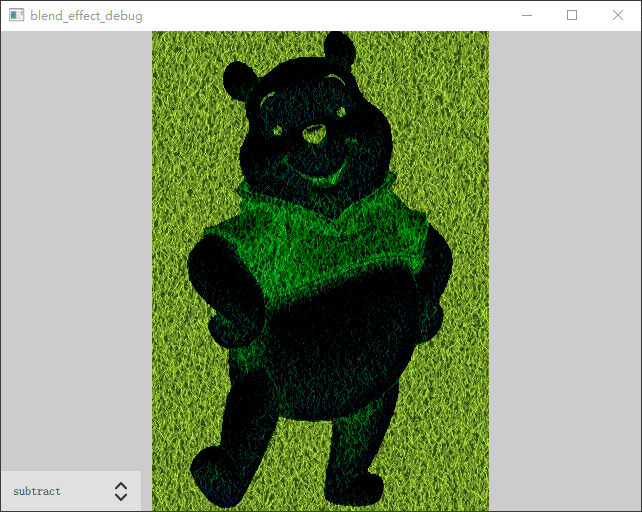
\includegraphics[width=0.95\textwidth]{../chapter06/blend_effect/the_app.png} %图片路径
\caption{Blend} %标题
\label{p000018} %索引
\end{figure}
%end图片


%\begin{spacing}{1.0}
\refstepcounter{filesourcenumber}\label{f000052}    %增加源代码编号
\FloatBarrier                                  %强制完成浮动体布局
\begin{thebookfilesourceone}[escapeinside={(*@}{@*)},
caption=GoodLuck,
title=\filesourcenumbernameone \thefilesourcenumber
]
/*blend_effect/main.qml*/
import QtQuick 2.9
import QtGraphicalEffects 1.12

Rectangle {
    id : idRoot
    width: 640;
    height: 480;
    color: Qt.rgba(0.8,0.8,0.8,1);

    Image{
        anchors.fill: idBear;
        source: "grass.jpg"
        fillMode: Image.Tile
        id : idGrass
        visible: false
    }

    Image{
        anchors.centerIn: parent;
        source: "bear.png"
        fillMode: Image.Stretch
        id : idBear
        visible: false
    }

    Blend{
        source: idGrass
        foregroundSource: idBear
        mode: idBlendControl.blendModeComboBox.currentText
        anchors.centerIn: parent;
        width: idBear.width
        height: idBear.height
    }

    BlendControl {
        id : idBlendControl
    }

}(*@\marginpar[\hfill\setlength\fboxsep{2pt}\fbox{\footnotesize{\kaishu\parbox{1em}{\setlength{\baselineskip}{2pt}\filesourcenumbernameone}}\footnotesize{\thefilesourcenumber}}]{\setlength\fboxsep{2pt}\fbox{\footnotesize{\kaishu\parbox{1em}{\setlength{\baselineskip}{2pt}\filesourcenumbernameone}}\footnotesize{\thefilesourcenumber}}}@*)\end{thebookfilesourceone}          %抄录环境
\addtocounter{lstlisting}{-1}   %sub lstlisting counter ...
%\end{spacing}






%使用XeLaTeX编译
%版权所有,翻版必究
%本文件由程序自动生成,任何修改将被覆盖
%2019 年 01 月 23 日





%使用XeLaTeX编译
%版权所有,翻版必究
%本文件由程序自动生成,任何修改将被覆盖
%2019 年 01 月 23 日





\begin{comment}
#version 150 core
in vec2 qt_TexCoord0;
uniform float qt_Opacity;
uniform sampler2D source;
uniform float brightness;
uniform float contrast;
out vec4 fragColor;

void main() {
    vec4 pixelColor = texture(source, qt_TexCoord0);
    pixelColor.rgb /= max(1.0/256.0, pixelColor.a);
    float c = 1.0 + contrast;
    float contrastGainFactor = 1.0 + c * c * c * c * step(0.0, contrast);
    pixelColor.rgb = ((pixelColor.rgb - 0.5) * (contrastGainFactor * contrast + 1.0)) + 0.5;
    pixelColor.rgb = mix(pixelColor.rgb, vec3(step(0.0, brightness)), abs(brightness));
    fragColor = vec4(pixelColor.rgb * pixelColor.a, pixelColor.a) * qt_Opacity;
}
\end{comment}


\FloatBarrier
\section{
BrightnessContrast
}\label{c000015s000003}


BrightnessContrast用于调整亮度和对比度。其常见属性
见\tablename\ \ref{tb000003}。


%使用XeLaTeX编译
%版权所有,翻版必究
%本文件由程序自动生成,任何修改将被覆盖
%2019 年 01 月 23 日



%表
\begin{longtable}{ccc}

%表头....
\toprule{}类名 
&
分类
&
简介%there must use marginnote ...
\marginnote{\setlength\fboxsep{2pt}\fbox{\footnotesize{\kaishu\tablename\,}\footnotesize{\ref{tb000000}}}}
\\ \midrule 
\endfirsthead

%表尾...
\bottomrule
\caption{ThresholdMask}\label{tb000000} 
\endlastfoot

%重复表头
\toprule{}类名 
&
分类
&
简介
\\ \midrule
\endhead
%重复表尾
\midrule
\endfoot 
Blend & aabbc & cccc \\
BrightnessContrast & aabbc & cccc \\
ColorOverlay & aabbc & cccc \\
Colorize & aabbc & cccc \\
Desaturate & aabbc & cccc \\
GammaAdjust & aabbc & cccc \\
HueSaturation & aabbc & cccc \\
LevelAdjust & aabbc & cccc \\
ConicalGradient & aabbc & cccc \\
LinearGradient & aabbc & cccc \\
RadialGradient & aabbc & cccc \\
Displace & aabbc & cccc \\
DropShadow & aabbc & cccc \\
InnerShadow & aabbc & cccc \\
FastBlur & aabbc & cccc \\
GaussianBlur & aabbc & cccc \\
MaskedBlur & aabbc & cccc \\
RecursiveBlur & aabbc & cccc \\
DirectionalBlur & aabbc & cccc \\
RadialBlur & aabbc & cccc \\
ZoomBlur & aabbc & cccc \\
Glow & aabbc & cccc \\
RectangularGlow & aabbc & cccc \\
OpacityMask & aabbc & cccc \\
ThresholdMask  & aabbc & cccc \\
\end{longtable}
%表





%使用XeLaTeX编译
%版权所有,翻版必究
%本文件由程序自动生成,任何修改将被覆盖
%2019 年 01 月 23 日





BrightnessContrast的关键代码
见\filesourcenumbernameone\ \ref{f000077}。
%\begin{spacing}{1.0}
\refstepcounter{filesourcenumber}\label{f000077}    %增加源代码编号
\FloatBarrier                                  %强制完成浮动体布局
\begin{thebookfilesourceone}[escapeinside={(*@}{@*)},
caption=GoodLuck,
title=\filesourcenumbernameone \thefilesourcenumber
]
/*+glslcore/brightnesscontrast.frag*/
#version 150 core
in vec2 qt_TexCoord0;
uniform float qt_Opacity;
uniform sampler2D source;
uniform float brightness;
uniform float contrast;
out vec4 fragColor;

void main() {
    vec4 pixelColor = texture(source, qt_TexCoord0);
    pixelColor.rgb /= max(1.0/256.0, pixelColor.a);
    float c = 1.0 + contrast;
    float contrastGainFactor = 1.0 + c * c * c * c * step(0.0, contrast);
    pixelColor.rgb =
        ((pixelColor.rgb - 0.5) * (contrastGainFactor * contrast + 1.0)) + 0.5;
    pixelColor.rgb =
        mix(pixelColor.rgb, vec3(step(0.0, brightness)), abs(brightness));
    fragColor = vec4(pixelColor.rgb * pixelColor.a, pixelColor.a) * qt_Opacity;
}(*@\marginpar[\hfill\setlength\fboxsep{2pt}\fbox{\footnotesize{\kaishu\parbox{1em}{\setlength{\baselineskip}{2pt}\filesourcenumbernameone}}\footnotesize{\thefilesourcenumber}}]{\setlength\fboxsep{2pt}\fbox{\footnotesize{\kaishu\parbox{1em}{\setlength{\baselineskip}{2pt}\filesourcenumbernameone}}\footnotesize{\thefilesourcenumber}}}@*)\end{thebookfilesourceone}          %抄录环境
\addtocounter{lstlisting}{-1}   %sub lstlisting counter ...
%\end{spacing}


本节案例源码见\filesourcenumbernameone\ \ref{f000053}。

%begin图片
\begin{figure}[htb] %浮动体 here and top ...
%there must use marginnote ...
\marginnote{\setlength\fboxsep{2pt}\fbox{\footnotesize{\kaishu\figurename\,}\footnotesize{\ref{p000019}}}}\centering %中心对齐
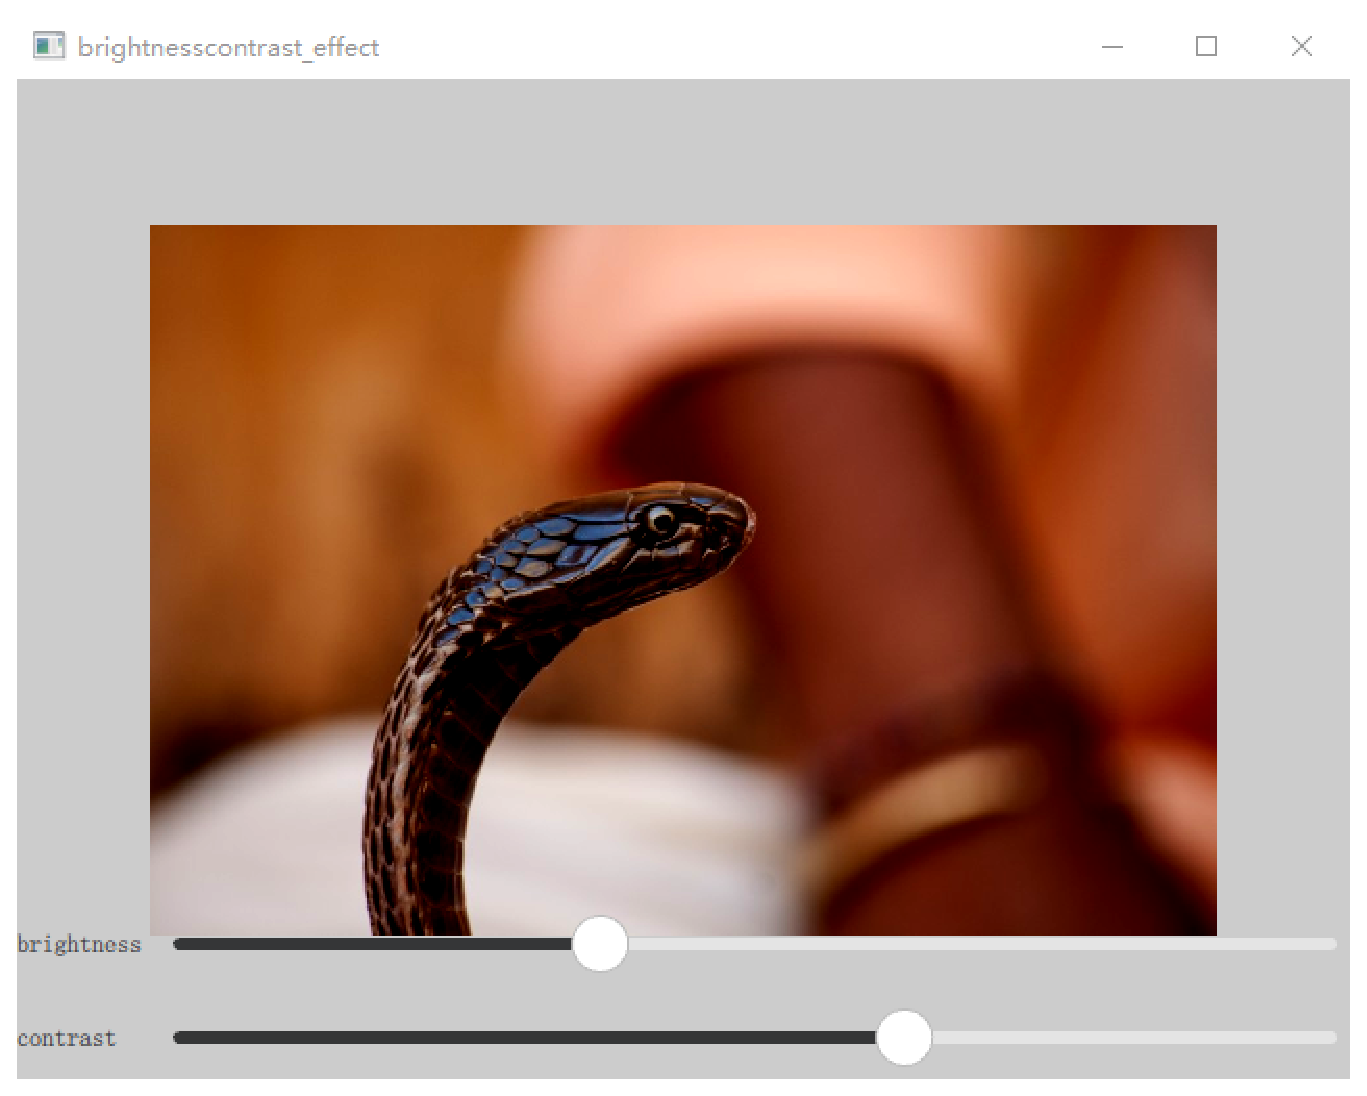
\includegraphics[width=0.95\textwidth]{the_book_image/p000019.eps} %图片路径
\caption{BrightnessContrast} %标题
\label{p000019} %索引
\end{figure}
%end图片


%\begin{spacing}{1.0}
\refstepcounter{filesourcenumber}\label{f000053}    %增加源代码编号
\FloatBarrier                                  %强制完成浮动体布局
\begin{thebookfilesourceone}[escapeinside={(*@}{@*)},
caption=GoodLuck,
title=\filesourcenumbernameone \thefilesourcenumber
]
/*brightnesscontrast_effect/main.qml*/
import QtQuick 2.9
import QtGraphicalEffects 1.12

Rectangle {

    id : idRoot
    width: 640;
    height: 480;
    color: Qt.rgba(0.8,0.8,0.8,1);


    Image{
        width: parent.width * 0.8;
        height: parent.height * 0.8;
        anchors.centerIn: parent
        source: "image.jpg"
        visible: false
        fillMode: Image.PreserveAspectFit
        id : idImage
    }

    BrightnessContrast{
        anchors.fill: idImage
        source: idImage
        contrast: idControl.contrastItem.value
        brightness: idControl.brightnessItem.value
    }

    BrightnessContrastControl{
        id:idControl
    }

}(*@\marginpar[\hfill\setlength\fboxsep{2pt}\fbox{\footnotesize{\kaishu\parbox{1em}{\setlength{\baselineskip}{2pt}\filesourcenumbernameone}}\footnotesize{\thefilesourcenumber}}]{\setlength\fboxsep{2pt}\fbox{\footnotesize{\kaishu\parbox{1em}{\setlength{\baselineskip}{2pt}\filesourcenumbernameone}}\footnotesize{\thefilesourcenumber}}}@*)\end{thebookfilesourceone}          %抄录环境
\addtocounter{lstlisting}{-1}   %sub lstlisting counter ...
%\end{spacing}



























%使用XeLaTeX编译
%版权所有,翻版必究
%本文件由程序自动生成,任何修改将被覆盖
%2019 年 01 月 23 日





%使用XeLaTeX编译
%版权所有,翻版必究
%本文件由程序自动生成,任何修改将被覆盖
%2019 年 01 月 23 日




\FloatBarrier
\section{
ColorOverlay
}\label{c000015s000004}


ColorOverlay用于在可渲染对象上叠加一个颜色。其常见属性
见\tablename\ \ref{tb000003}。


%使用XeLaTeX编译
%版权所有,翻版必究
%本文件由程序自动生成,任何修改将被覆盖
%2019 年 01 月 23 日



%表
\begin{longtable}{ccc}

%表头....
\toprule{}类名 
&
分类
&
简介%there must use marginnote ...
\marginnote{\setlength\fboxsep{2pt}\fbox{\footnotesize{\kaishu\tablename\,}\footnotesize{\ref{tb000000}}}}
\\ \midrule 
\endfirsthead

%表尾...
\bottomrule
\caption{ThresholdMask}\label{tb000000} 
\endlastfoot

%重复表头
\toprule{}类名 
&
分类
&
简介
\\ \midrule
\endhead
%重复表尾
\midrule
\endfoot 
Blend & aabbc & cccc \\
BrightnessContrast & aabbc & cccc \\
ColorOverlay & aabbc & cccc \\
Colorize & aabbc & cccc \\
Desaturate & aabbc & cccc \\
GammaAdjust & aabbc & cccc \\
HueSaturation & aabbc & cccc \\
LevelAdjust & aabbc & cccc \\
ConicalGradient & aabbc & cccc \\
LinearGradient & aabbc & cccc \\
RadialGradient & aabbc & cccc \\
Displace & aabbc & cccc \\
DropShadow & aabbc & cccc \\
InnerShadow & aabbc & cccc \\
FastBlur & aabbc & cccc \\
GaussianBlur & aabbc & cccc \\
MaskedBlur & aabbc & cccc \\
RecursiveBlur & aabbc & cccc \\
DirectionalBlur & aabbc & cccc \\
RadialBlur & aabbc & cccc \\
ZoomBlur & aabbc & cccc \\
Glow & aabbc & cccc \\
RectangularGlow & aabbc & cccc \\
OpacityMask & aabbc & cccc \\
ThresholdMask  & aabbc & cccc \\
\end{longtable}
%表





%使用XeLaTeX编译
%版权所有,翻版必究
%本文件由程序自动生成,任何修改将被覆盖
%2019 年 01 月 23 日






%    file:///G:/qt-everywhere-src-5.12.0/qtgraphicaleffects/src/effects/shaders/+glslcore/coloroverlay.frag


ColorOverlay的关键代码
见\filesourcenumbernameone\ \ref{f000078}。
%\begin{spacing}{1.0}
\refstepcounter{filesourcenumber}\label{f000078}    %增加源代码编号
\FloatBarrier                                  %强制完成浮动体布局
\begin{thebookfilesourceone}[escapeinside={(*@}{@*)},
caption=GoodLuck,
title=\filesourcenumbernameone \thefilesourcenumber
]
/*+glslcore/coloroverlay.frag*/
#version 150 core
in vec2 qt_TexCoord0;
uniform float qt_Opacity;
uniform sampler2D source;
uniform vec4 color;
out vec4 fragColor;
void main() {
    vec4 pixelColor = texture(source, qt_TexCoord0);
    fragColor = vec4(
        mix(pixelColor.rgb/max(pixelColor.a, 0.00390625),
            color.rgb/max(color.a, 0.00390625),
            color.a) * pixelColor.a,
        pixelColor.a) * qt_Opacity;
}(*@\marginpar[\hfill\setlength\fboxsep{2pt}\fbox{\footnotesize{\kaishu\parbox{1em}{\setlength{\baselineskip}{2pt}\filesourcenumbernameone}}\footnotesize{\thefilesourcenumber}}]{\setlength\fboxsep{2pt}\fbox{\footnotesize{\kaishu\parbox{1em}{\setlength{\baselineskip}{2pt}\filesourcenumbernameone}}\footnotesize{\thefilesourcenumber}}}@*)\end{thebookfilesourceone}          %抄录环境
\addtocounter{lstlisting}{-1}   %sub lstlisting counter ...
%\end{spacing}


本节案例源码见\filesourcenumbernameone\ \ref{f000054}。

%begin图片
\begin{figure}[htb] %浮动体 here and top ...
%there must use marginnote ...
\marginnote{\setlength\fboxsep{2pt}\fbox{\footnotesize{\kaishu\figurename\,}\footnotesize{\ref{p000020}}}}\centering %中心对齐
\setlength\fboxsep{0pt}\fcolorbox[rgb]{0,0,0}{0.97,0.98,0.99}{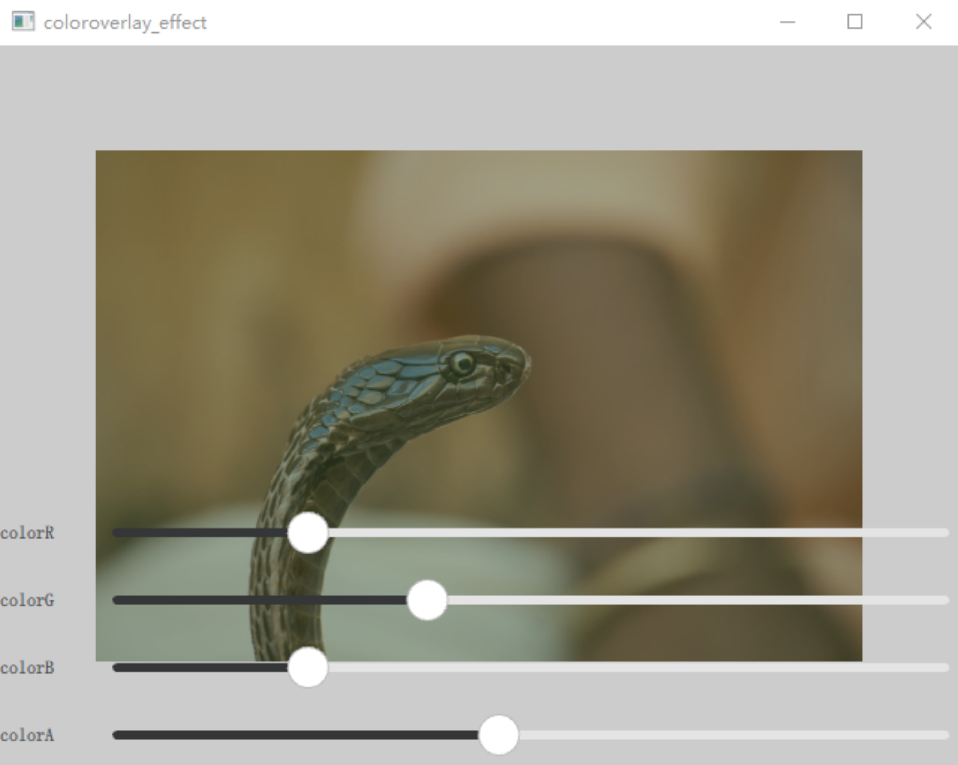
\includegraphics[width=0.95\textwidth]{the_book_image/p000020.pdf}} %图片路径
\caption{ColorOverlay} %标题
\label{p000020} %索引
\end{figure}
%end图片


%\begin{spacing}{1.0}
\refstepcounter{filesourcenumber}\label{f000054}    %增加源代码编号
\FloatBarrier                                  %强制完成浮动体布局
\begin{thebookfilesourceone}[escapeinside={(*@}{@*)},
caption=GoodLuck,
title=\filesourcenumbernameone \thefilesourcenumber
]
/*coloroverlay_effect/main.qml*/
import QtQuick 2.9
import QtGraphicalEffects 1.12

Rectangle {

    id : idRoot
    width: 640;
    height: 480;
    color: Qt.rgba(0.8,0.8,0.8,1);

    Image{
        width: parent.width * 0.8;
        height: parent.height * 0.8;
        anchors.centerIn: parent
        source: "image.jpg"
        visible: false
        fillMode: Image.PreserveAspectFit
        id : idImage
    }

    ColorOverlay{
        anchors.fill: idImage
        source: idImage
        color: idColoroverlayControl.applyColor
    }

    ColoroverlayControl{
        id : idColoroverlayControl
    }

}(*@\marginpar[\hfill\setlength\fboxsep{2pt}\fbox{\footnotesize{\kaishu\parbox{1em}{\setlength{\baselineskip}{2pt}\filesourcenumbernameone}}\footnotesize{\thefilesourcenumber}}]{\setlength\fboxsep{2pt}\fbox{\footnotesize{\kaishu\parbox{1em}{\setlength{\baselineskip}{2pt}\filesourcenumbernameone}}\footnotesize{\thefilesourcenumber}}}@*)\end{thebookfilesourceone}          %抄录环境
\addtocounter{lstlisting}{-1}   %sub lstlisting counter ...
%\end{spacing}


 






%使用XeLaTeX编译
%版权所有,翻版必究
%本文件由程序自动生成,任何修改将被覆盖
%2019 年 01 月 23 日





%使用XeLaTeX编译
%版权所有,翻版必究
%本文件由程序自动生成,任何修改将被覆盖
%2019 年 01 月 23 日




\FloatBarrier
\section{
Colorize
}\label{c000015s000005}


%begin图片
\begin{figure}[htb] %浮动体 here and top ...
%there must use marginnote ...
\marginnote{\setlength\fboxsep{2pt}\fbox{\footnotesize{\kaishu\figurename\,}\footnotesize{\ref{p000021}}}}\centering %中心对齐
\setlength\fboxsep{0pt}\fcolorbox[rgb]{0,0,0}{0.97,0.98,0.99}{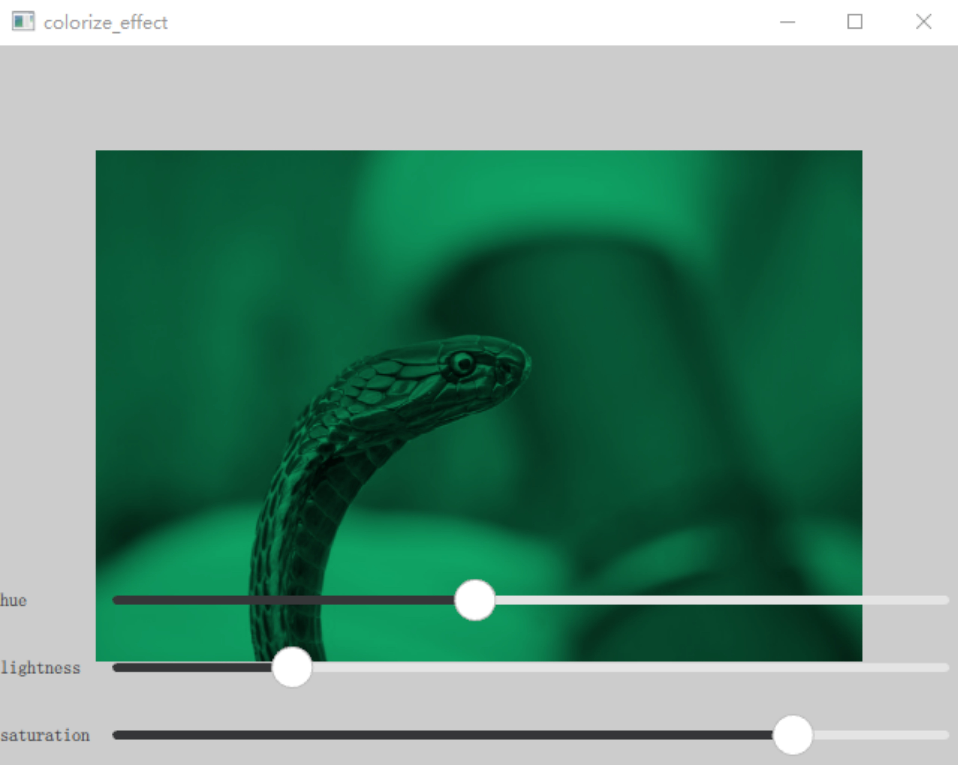
\includegraphics[width=0.95\textwidth]{the_book_image/p000021.pdf}} %图片路径
\caption{Colorize} %标题
\label{p000021} %索引
\end{figure}
%end图片


%\begin{spacing}{1.0}
\refstepcounter{filesourcenumber}\label{f000055}    %增加源代码编号
\FloatBarrier                                  %强制完成浮动体布局
\begin{thebookfilesourceone}[escapeinside={(*@}{@*)},
caption=GoodLuck,
title=\filesourcenumbernameone \thefilesourcenumber
]
/*colorize_effect/main.qml*/
import QtQuick 2.9
import QtGraphicalEffects 1.12

Rectangle {

    id : idRoot
    width: 640;
    height: 480;
    color: Qt.rgba(0.8,0.8,0.8,1);

    Image{
        width: parent.width * 0.8;
        height: parent.height * 0.8;
        anchors.centerIn: parent
        source: "image.jpg"
        visible: false
        fillMode: Image.PreserveAspectFit
        id : idImage
    }

    Colorize {
        anchors.fill: idImage
        source: idImage
        hue: idColorizeControl.hueItem.value;
        lightness: idColorizeControl.lightnessItem.value;
        saturation: idColorizeControl.saturationItem.value;
    }

    ColorizeControl{
        id : idColorizeControl
    }

}(*@\marginpar[\hfill\setlength\fboxsep{2pt}\fbox{\footnotesize{\kaishu\parbox{1em}{\setlength{\baselineskip}{2pt}\filesourcenumbernameone}}\footnotesize{\thefilesourcenumber}}]{\setlength\fboxsep{2pt}\fbox{\footnotesize{\kaishu\parbox{1em}{\setlength{\baselineskip}{2pt}\filesourcenumbernameone}}\footnotesize{\thefilesourcenumber}}}@*)\end{thebookfilesourceone}          %抄录环境
\addtocounter{lstlisting}{-1}   %sub lstlisting counter ...
%\end{spacing}


未完待续


% ______all_key_words
% the_book_chapter the_book_subsection the_book_subsubsection
% the_book_section the_book_image the_book_table
% the_book_file the_book_tree_file the_book_command_file
% littlelongworld tabbing ref
% figurename tablename filesourcenumbernameone
% treeindexnumbernameone commandnumbernameone footnote 
% item itemize comment textbullet
% \hspace*{\parindent}







%使用XeLaTeX编译
%版权所有,翻版必究
%本文件由程序自动生成,任何修改将被覆盖
%2019 年 01 月 23 日





%使用XeLaTeX编译
%版权所有,翻版必究
%本文件由程序自动生成,任何修改将被覆盖
%2019 年 01 月 23 日




\FloatBarrier
\section{
Desaturate
}\label{c000015s000006}


%begin图片
\begin{figure}[htb] %浮动体 here and top ...
%there must use marginnote ...
\marginnote{\setlength\fboxsep{2pt}\fbox{\footnotesize{\kaishu\figurename\,}\footnotesize{\ref{p000022}}}}\centering %中心对齐
\setlength\fboxsep{0pt}\fcolorbox[rgb]{0,0,0}{0,0,0}{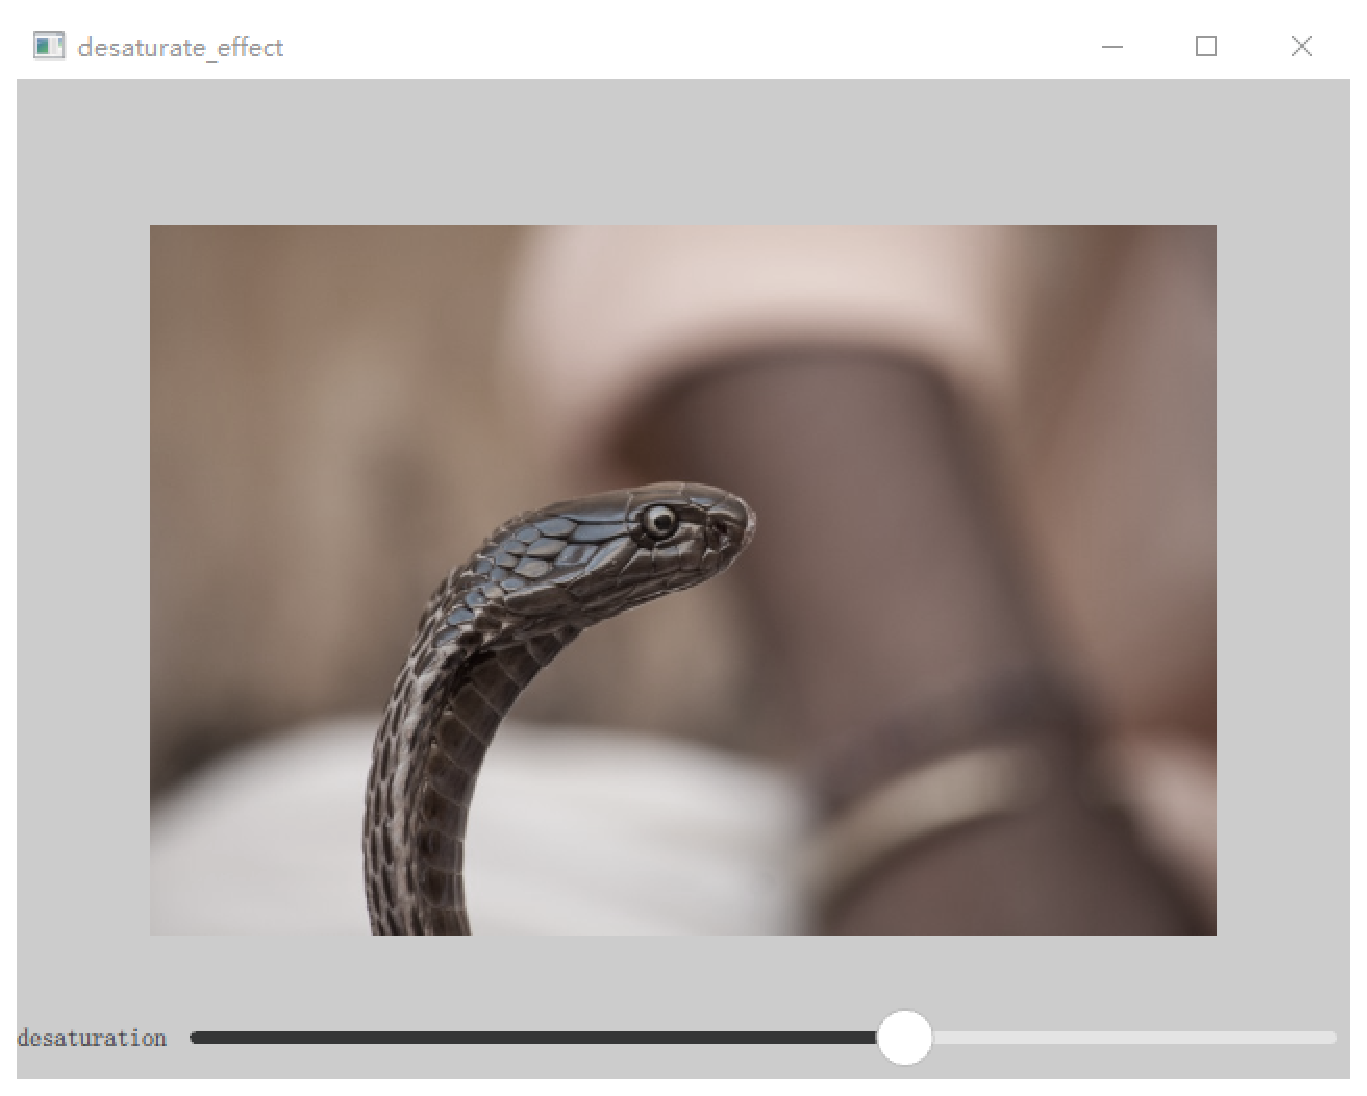
\includegraphics[width=0.95\textwidth]{the_book_image/p000022.eps}} %图片路径
\caption{Desaturate} %标题
\label{p000022} %索引
\end{figure}
%end图片


%\begin{spacing}{1.0}
\refstepcounter{filesourcenumber}\label{f000056}    %增加源代码编号
\FloatBarrier                                  %强制完成浮动体布局
\begin{thebookfilesourceone}[escapeinside={(*@}{@*)},
caption=GoodLuck,
title=\filesourcenumbernameone \thefilesourcenumber
]
/*desaturate_effect/main.qml*/
import QtQuick 2.9
import QtGraphicalEffects 1.12

Rectangle {

    id : idRoot
    width: 640;
    height: 480;
    color: Qt.rgba(0.8,0.8,0.8,1);

    Image{
        width: parent.width * 0.8;
        height: parent.height * 0.8;
        anchors.centerIn: parent
        source: "image.jpg"
        visible: false
        fillMode: Image.PreserveAspectFit
        id : idImage
    }

    Desaturate{
        anchors.fill: idImage
        source: idImage
        desaturation: thisControl.desaturationItem.value
    }

    DesaturateControl{
        id : thisControl
    }

}(*@\marginpar[\hfill\setlength\fboxsep{2pt}\fbox{\footnotesize{\kaishu\parbox{1em}{\setlength{\baselineskip}{2pt}\filesourcenumbernameone}}\footnotesize{\thefilesourcenumber}}]{\setlength\fboxsep{2pt}\fbox{\footnotesize{\kaishu\parbox{1em}{\setlength{\baselineskip}{2pt}\filesourcenumbernameone}}\footnotesize{\thefilesourcenumber}}}@*)\end{thebookfilesourceone}          %抄录环境
\addtocounter{lstlisting}{-1}   %sub lstlisting counter ...
%\end{spacing}


未完待续






%使用XeLaTeX编译
%版权所有,翻版必究
%本文件由程序自动生成,任何修改将被覆盖
%2019 年 01 月 23 日





%使用XeLaTeX编译
%版权所有,翻版必究
%本文件由程序自动生成,任何修改将被覆盖
%2019 年 01 月 23 日




\FloatBarrier
\section{
GammaAdjust
}\label{c000015s000007}


%begin图片
\begin{figure}[htb] %浮动体 here and top ...
%there must use marginnote ...
\marginnote{\setlength\fboxsep{2pt}\fbox{\footnotesize{\kaishu\figurename\,}\footnotesize{\ref{p000023}}}}\centering %中心对齐
\setlength\fboxsep{0pt}\fcolorbox[rgb]{0,0,0}{0,0,0}{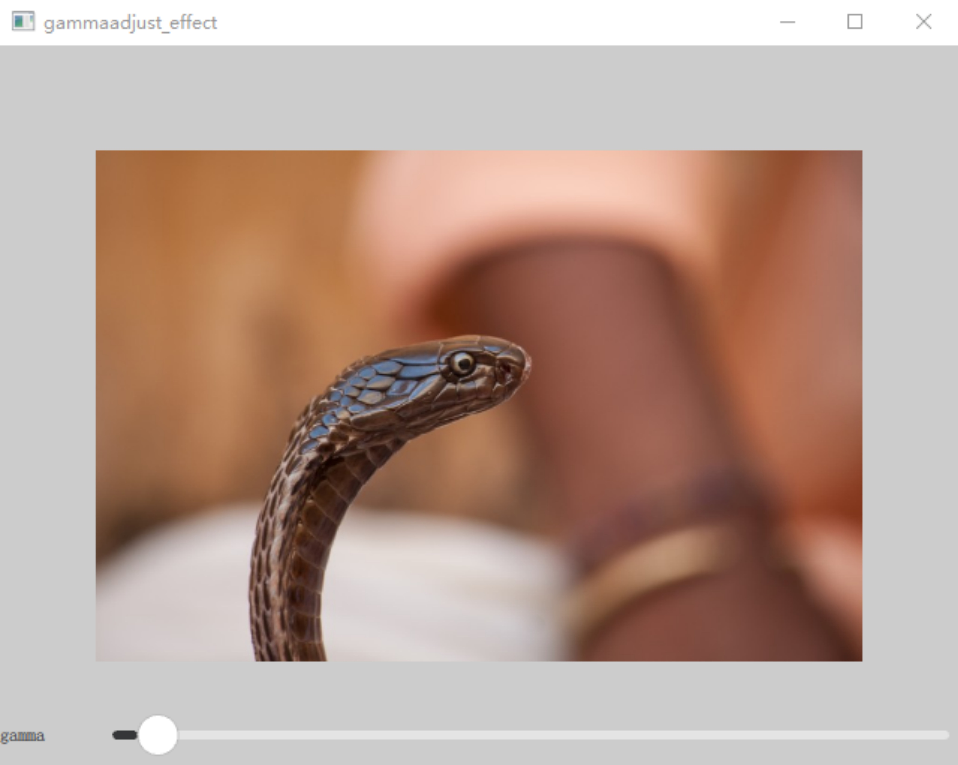
\includegraphics[width=0.95\textwidth]{the_book_image/p000023.pdf}} %图片路径
\caption{GammaAdjust} %标题
\label{p000023} %索引
\end{figure}
%end图片


%\begin{spacing}{1.0}
\refstepcounter{filesourcenumber}\label{f000057}    %增加源代码编号
\FloatBarrier                                  %强制完成浮动体布局
\begin{thebookfilesourceone}[escapeinside={(*@}{@*)},
caption=GoodLuck,
title=\filesourcenumbernameone \thefilesourcenumber
]
/*gammaadjust_effect/main.qml*/
import QtQuick 2.9
import QtGraphicalEffects 1.12

Rectangle {
    id : idRoot
    width: 640;
    height: 480;
    color: Qt.rgba(0.8,0.8,0.8,1);

    Image{
        width: parent.width * 0.8;
        height: parent.height * 0.8;
        anchors.centerIn: parent
        source: "image"
        visible: false
        fillMode: Image.PreserveAspectFit
        id : idImage
    }

    GammaAdjust{
        anchors.fill: idImage
        source: idImage
        gamma: idThisControl.gammaItem.value
    }

    GammaAdjustControl{
        id : idThisControl
    }

}(*@\marginpar[\hfill\setlength\fboxsep{2pt}\fbox{\footnotesize{\kaishu\parbox{1em}{\setlength{\baselineskip}{2pt}\filesourcenumbernameone}}\footnotesize{\thefilesourcenumber}}]{\setlength\fboxsep{2pt}\fbox{\footnotesize{\kaishu\parbox{1em}{\setlength{\baselineskip}{2pt}\filesourcenumbernameone}}\footnotesize{\thefilesourcenumber}}}@*)\end{thebookfilesourceone}          %抄录环境
\addtocounter{lstlisting}{-1}   %sub lstlisting counter ...
%\end{spacing}


未完待续






%使用XeLaTeX编译
%版权所有,翻版必究
%本文件由程序自动生成,任何修改将被覆盖
%2019 年 01 月 23 日





%使用XeLaTeX编译
%版权所有,翻版必究
%本文件由程序自动生成,任何修改将被覆盖
%2019 年 01 月 23 日




\FloatBarrier
\section{
HueSaturation
}\label{c000015s000008}


%begin图片
\begin{figure}[htb] %浮动体 here and top ...
%there must use marginnote ...
\marginnote{\setlength\fboxsep{2pt}\fbox{\footnotesize{\kaishu\figurename\,}\footnotesize{\ref{p000024}}}}\centering %中心对齐
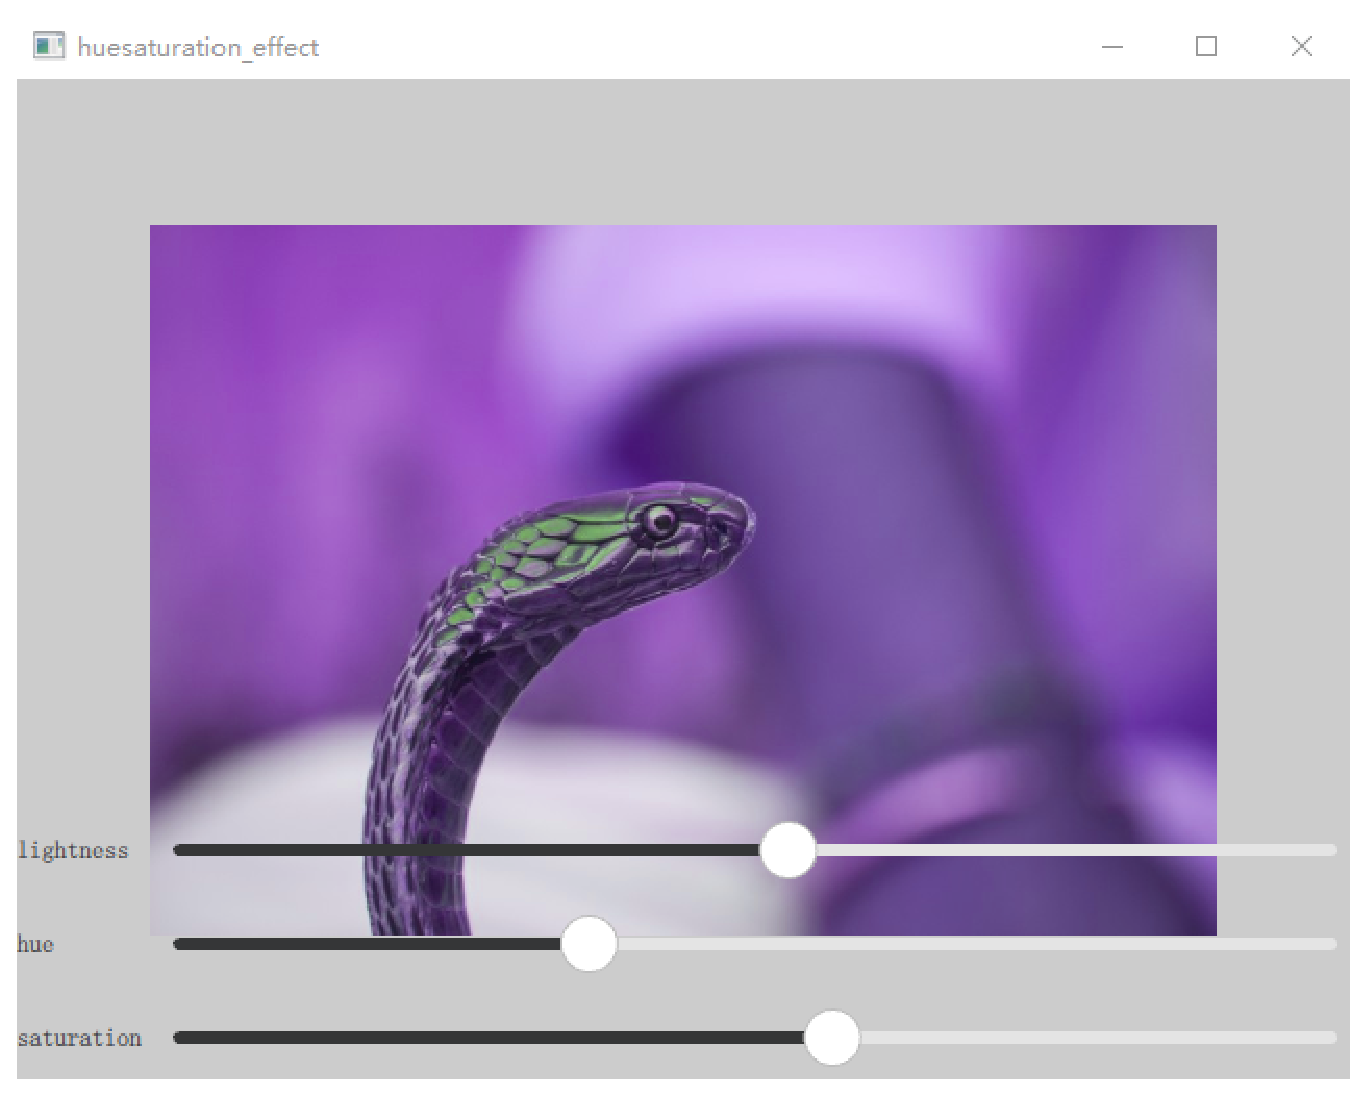
\includegraphics[width=0.95\textwidth]{the_book_image/p000024.eps} %图片路径
\caption{HueSaturation} %标题
\label{p000024} %索引
\end{figure}
%end图片


%\begin{spacing}{1.0}
\refstepcounter{filesourcenumber}\label{f000058}    %增加源代码编号
\FloatBarrier                                  %强制完成浮动体布局
\begin{thebookfilesourceone}[escapeinside={(*@}{@*)},
caption=GoodLuck,
title=\filesourcenumbernameone \thefilesourcenumber
]
/*huesaturation_effect/main.qml*/
import QtQuick 2.9
import QtGraphicalEffects 1.12

Rectangle {
    id : idRoot
    width: 640;
    height: 480;
    color: Qt.rgba(0.8,0.8,0.8,1);

    Image{
        width: parent.width * 0.8;
        height: parent.height * 0.8;
        anchors.centerIn: parent
        source: "image"
        visible: false
        fillMode: Image.PreserveAspectFit
        id : idImage
    }

    HueSaturation{
        anchors.fill: idImage
        source: idImage
        hue : thisControl.hueItem.value
        lightness: thisControl.lightnessItem.value
        saturation: thisControl.saturationItem.value
    }

    HuesaturationControl{
        id : thisControl
    }

}(*@\marginpar[\hfill\setlength\fboxsep{2pt}\fbox{\footnotesize{\kaishu\parbox{1em}{\setlength{\baselineskip}{2pt}\filesourcenumbernameone}}\footnotesize{\thefilesourcenumber}}]{\setlength\fboxsep{2pt}\fbox{\footnotesize{\kaishu\parbox{1em}{\setlength{\baselineskip}{2pt}\filesourcenumbernameone}}\footnotesize{\thefilesourcenumber}}}@*)\end{thebookfilesourceone}          %抄录环境
\addtocounter{lstlisting}{-1}   %sub lstlisting counter ...
%\end{spacing}


未完待续






%使用XeLaTeX编译
%版权所有,翻版必究
%本文件由程序自动生成,任何修改将被覆盖
%2019 年 01 月 23 日





%使用XeLaTeX编译
%版权所有,翻版必究
%本文件由程序自动生成,任何修改将被覆盖
%2019 年 01 月 23 日




\FloatBarrier
\section{
LevelAdjust
}\label{c000015s000009}


%begin图片
\begin{figure}[htb] %浮动体 here and top ...
%there must use marginnote ...
\marginnote{\setlength\fboxsep{2pt}\fbox{\footnotesize{\kaishu\figurename\,}\footnotesize{\ref{p000025}}}}\centering %中心对齐
\setlength\fboxsep{0pt}\fcolorbox[rgb]{0,0,0}{0.97,0.98,0.99}{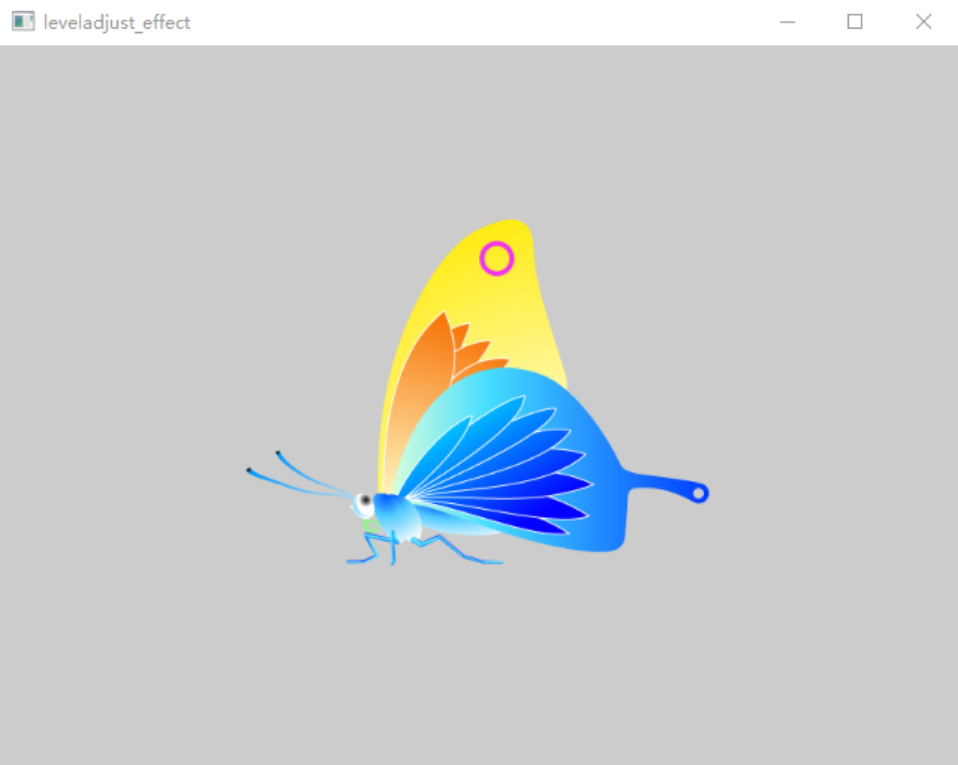
\includegraphics[width=0.95\textwidth]{the_book_image/p000025.pdf}} %图片路径
\caption{LevelAdjust} %标题
\label{p000025} %索引
\end{figure}
%end图片


%\begin{spacing}{1.0}
\refstepcounter{filesourcenumber}\label{f000059}    %增加源代码编号
\FloatBarrier                                  %强制完成浮动体布局
\begin{thebookfilesourceone}[escapeinside={(*@}{@*)},
caption=GoodLuck,
title=\filesourcenumbernameone \thefilesourcenumber
]
/*leveladjust_effect/main.qml*/
import QtQuick 2.9
import QtGraphicalEffects 1.12

Rectangle {
    id : idRoot
    width: 640;
    height: 480;
    color: Qt.rgba(0.8,0.8,0.8,1);

    Image{
        width: parent.width * 0.8;
        height: parent.height * 0.8;
        anchors.centerIn: parent
        source: "image"
        visible: false
        fillMode: Image.PreserveAspectFit
        id : idImage
    }

    /*将RGB反向,A不变*/
    LevelAdjust {
        anchors.fill: idImage
        source: idImage
        minimumOutput: Qt.rgba(1,1,1,0)
        maximumOutput: Qt.rgba(0,0,0,1)
    }

}(*@\marginpar[\hfill\setlength\fboxsep{2pt}\fbox{\footnotesize{\kaishu\parbox{1em}{\setlength{\baselineskip}{2pt}\filesourcenumbernameone}}\footnotesize{\thefilesourcenumber}}]{\setlength\fboxsep{2pt}\fbox{\footnotesize{\kaishu\parbox{1em}{\setlength{\baselineskip}{2pt}\filesourcenumbernameone}}\footnotesize{\thefilesourcenumber}}}@*)\end{thebookfilesourceone}          %抄录环境
\addtocounter{lstlisting}{-1}   %sub lstlisting counter ...
%\end{spacing}


未完待续


% ______all_key_words
% the_book_chapter the_book_subsection the_book_subsubsection
% the_book_section the_book_image the_book_table
% the_book_file the_book_tree_file the_book_command_file
% littlelongworld tabbing ref
% figurename tablename filesourcenumbernameone
% treeindexnumbernameone commandnumbernameone footnote 
% item itemize comment textbullet
% \hspace*{\parindent}







%使用XeLaTeX编译
%版权所有,翻版必究
%本文件由程序自动生成,任何修改将被覆盖
%2019 年 01 月 23 日





%使用XeLaTeX编译
%版权所有,翻版必究
%本文件由程序自动生成,任何修改将被覆盖
%2019 年 01 月 23 日




\FloatBarrier
\section{
ConicalGradient
}\label{c000015s000010}


%begin图片
\begin{figure}[htb] %浮动体 here and top ...
%there must use marginnote not use marginnote ...
\marginnote{\setlength\fboxsep{2pt}\fbox{\footnotesize{\kaishu\figurename\,}\footnotesize{\ref{p000026}}}}\centering %中心对齐
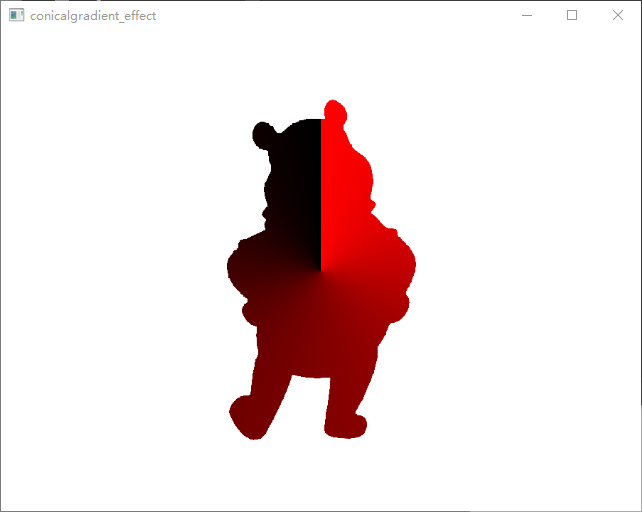
\includegraphics[width=0.95\textwidth]{../chapter06/conicalgradient_effect/the_app.png} %图片路径
\caption{ConicalGradient} %标题
\label{p000026} %索引
\end{figure}
%end图片


%\begin{spacing}{1.0}
\refstepcounter{filesourcenumber}\label{f000060}    %增加源代码编号
\FloatBarrier                                  %强制完成浮动体布局
\begin{thebookfilesourceone}[escapeinside={(*@}{@*)},
caption=GoodLuck,
title=\filesourcenumbernameone \thefilesourcenumber
]
/*conicalgradient_effect/main.qml*/
import QtQuick 2.9
import QtGraphicalEffects 1.12

Rectangle {
    id : idRoot
    width: 640;
    height: 480;

    Image{
        width: parent.width * 0.8;
        height: parent.height * 0.8;
        anchors.centerIn: parent
        source: "image.png"
        visible: false
        fillMode: Image.PreserveAspectFit
        id : idImage
    }

    ConicalGradient {
        anchors.fill: idImage
        source: idImage
        angle: 0.0
        gradient: Gradient {
            GradientStop { position: 0.0; color: "red" }
            GradientStop { position: 1.0; color: "black" }
        }
    }

}(*@\marginpar[\hfill\setlength\fboxsep{2pt}\fbox{\footnotesize{\kaishu\parbox{1em}{\setlength{\baselineskip}{2pt}\filesourcenumbernameone}}\footnotesize{\thefilesourcenumber}}]{\setlength\fboxsep{2pt}\fbox{\footnotesize{\kaishu\parbox{1em}{\setlength{\baselineskip}{2pt}\filesourcenumbernameone}}\footnotesize{\thefilesourcenumber}}}@*)\end{thebookfilesourceone}          %抄录环境
\addtocounter{lstlisting}{-1}   %sub lstlisting counter ...
%\end{spacing}


未完待续






%使用XeLaTeX编译
%版权所有,翻版必究
%本文件由程序自动生成,任何修改将被覆盖
%2019 年 01 月 23 日





%使用XeLaTeX编译
%版权所有,翻版必究
%本文件由程序自动生成,任何修改将被覆盖
%2019 年 01 月 23 日




\FloatBarrier
\section{
LinearGradient
}\label{c000015s000011}


%begin图片
\begin{figure}[htb] %浮动体 here and top ...
%there must use marginnote not use marginnote ...
\marginnote{\setlength\fboxsep{2pt}\fbox{\footnotesize{\kaishu\figurename\,}\footnotesize{\ref{p000027}}}}\centering %中心对齐
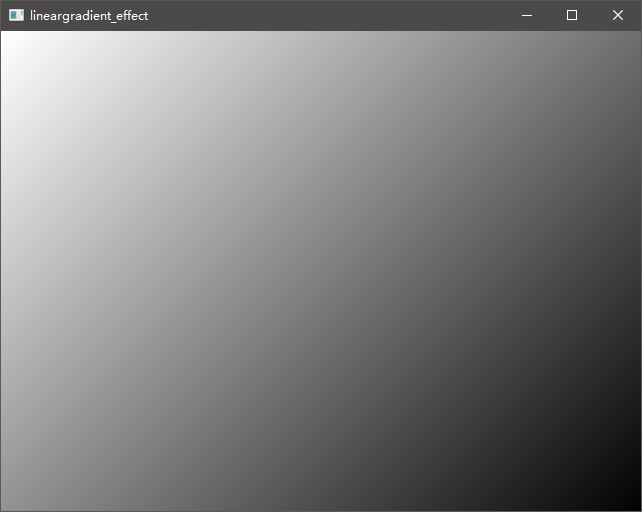
\includegraphics[width=0.95\textwidth]{../chapter06/lineargradient_effect/the_app.png} %图片路径
\caption{LinearGradient} %标题
\label{p000027} %索引
\end{figure}
%end图片


%\begin{spacing}{1.0}
\refstepcounter{filesourcenumber}\label{f000061}    %增加源代码编号
\FloatBarrier                                  %强制完成浮动体布局
\begin{thebookfilesourceone}[escapeinside={(*@}{@*)},
caption=GoodLuck,
title=\filesourcenumbernameone \thefilesourcenumber
]
/*lineargradient_effect/main.qml*/
import QtQuick 2.9
import QtGraphicalEffects 1.12

Rectangle {
    id : idRoot
    width: 640;
    height: 480;
    color: Qt.rgba(0.8,0.8,0.8,1);

    LinearGradient {
        id : idEffect
        anchors.fill: parent
        start: Qt.point(parent.x, parent.y)
        end: Qt.point(parent.x+parent.width,
                      parent.y+parent.height)
        gradient: Gradient {
            GradientStop { position: 0.0; color: "white" }
            GradientStop { position: 1.0; color: "black" }
        }
    }

}(*@\marginpar[\hfill\setlength\fboxsep{2pt}\fbox{\footnotesize{\kaishu\parbox{1em}{\setlength{\baselineskip}{2pt}\filesourcenumbernameone}}\footnotesize{\thefilesourcenumber}}]{\setlength\fboxsep{2pt}\fbox{\footnotesize{\kaishu\parbox{1em}{\setlength{\baselineskip}{2pt}\filesourcenumbernameone}}\footnotesize{\thefilesourcenumber}}}@*)\end{thebookfilesourceone}          %抄录环境
\addtocounter{lstlisting}{-1}   %sub lstlisting counter ...
%\end{spacing}


未完待续






%使用XeLaTeX编译
%版权所有,翻版必究
%本文件由程序自动生成,任何修改将被覆盖
%2019 年 01 月 23 日





%使用XeLaTeX编译
%版权所有,翻版必究
%本文件由程序自动生成,任何修改将被覆盖
%2019 年 01 月 23 日




\FloatBarrier
\section{
RadialGradient
}\label{c000015s000012}


%begin图片
\begin{figure}[htb] %浮动体 here and top ...
%there must use marginnote ...
\marginnote{\setlength\fboxsep{2pt}\fbox{\footnotesize{\kaishu\figurename\,}\footnotesize{\ref{p000028}}}}\centering %中心对齐
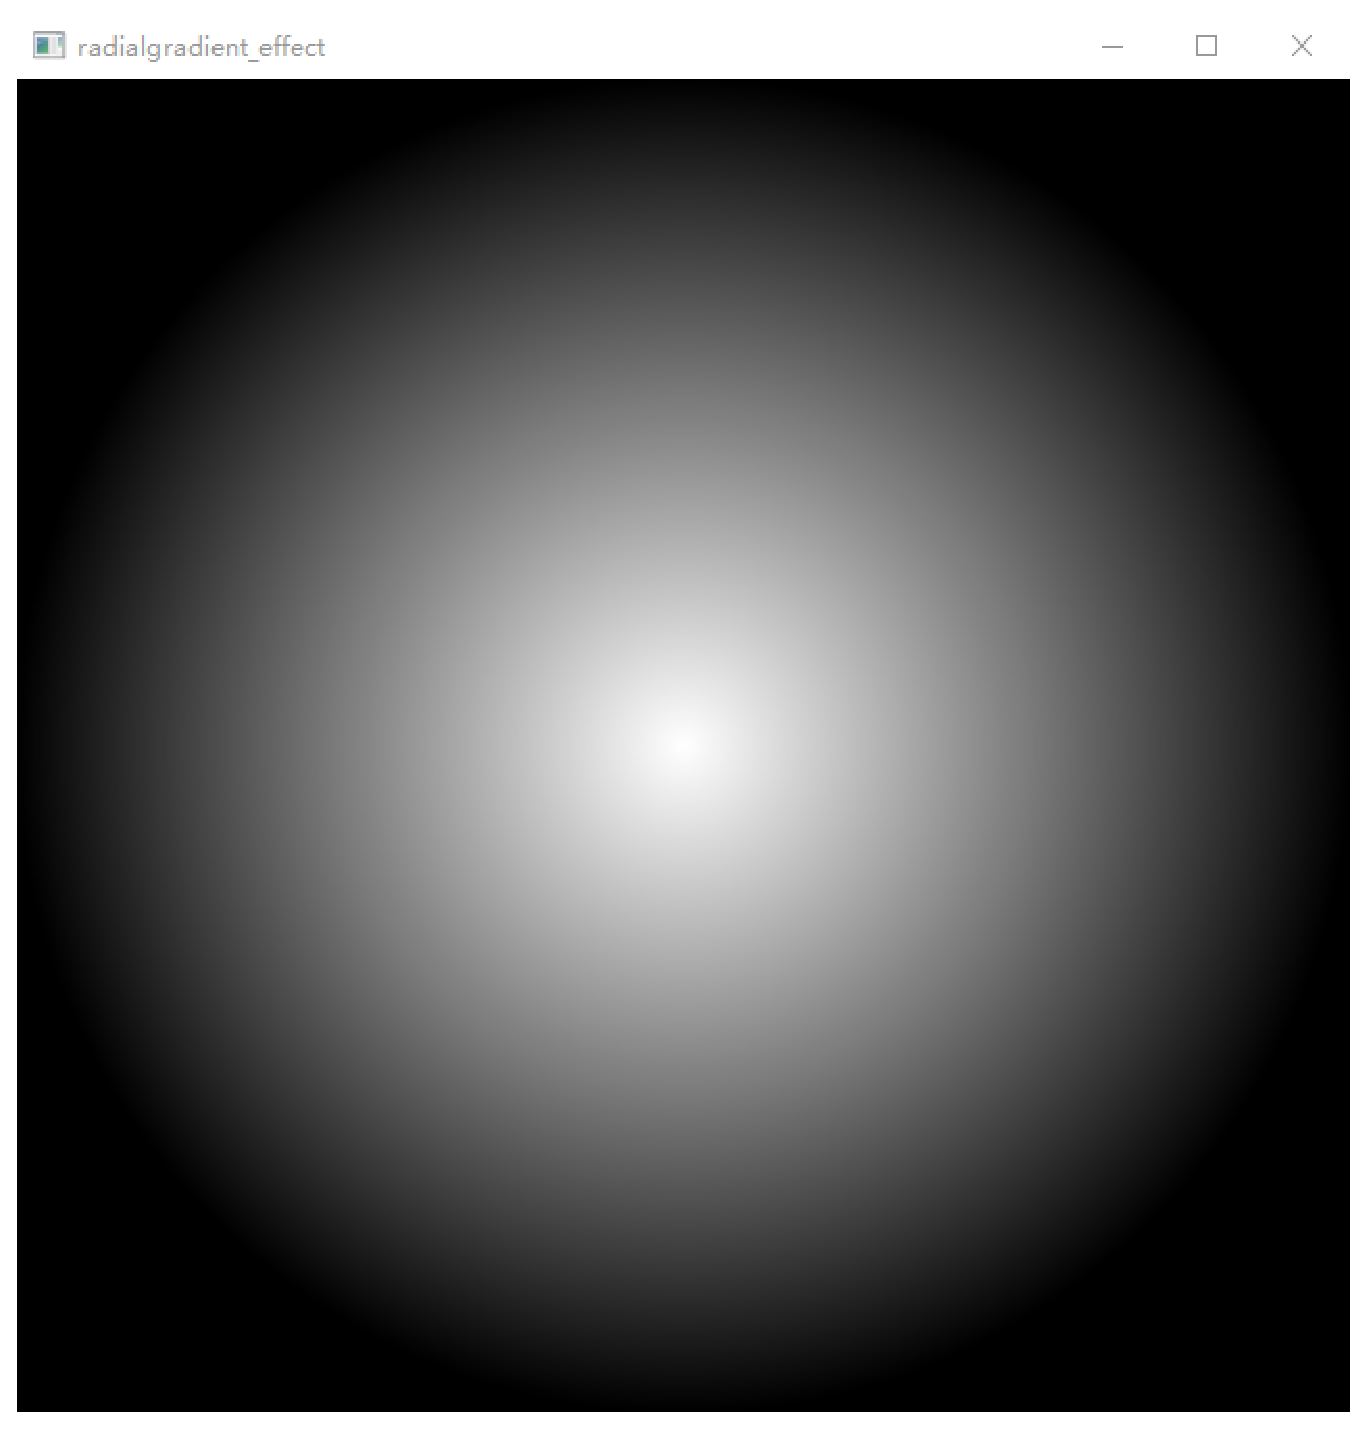
\includegraphics[width=0.95\textwidth]{the_book_image/p000028.eps} %图片路径
\caption{RadialGradient} %标题
\label{p000028} %索引
\end{figure}
%end图片


%\begin{spacing}{1.0}
\refstepcounter{filesourcenumber}\label{f000062}    %增加源代码编号
\FloatBarrier                                  %强制完成浮动体布局
\begin{thebookfilesourceone}[escapeinside={(*@}{@*)},
caption=GoodLuck,
title=\filesourcenumbernameone \thefilesourcenumber
]
/*radialgradient_effect/main.qml*/
import QtQuick 2.9
import QtGraphicalEffects 1.12

Rectangle {
    id : idRoot
    width: 640;
    height: 640;
    color: Qt.rgba(0.8,0.8,0.8,1);

    RadialGradient {
        anchors.fill: parent
        gradient: Gradient {
            GradientStop { position: 0.0; color: "white" }
            GradientStop { position: 0.5; color: "black" }
        }
    }

}(*@\marginpar[\hfill\setlength\fboxsep{2pt}\fbox{\footnotesize{\kaishu\parbox{1em}{\setlength{\baselineskip}{2pt}\filesourcenumbernameone}}\footnotesize{\thefilesourcenumber}}]{\setlength\fboxsep{2pt}\fbox{\footnotesize{\kaishu\parbox{1em}{\setlength{\baselineskip}{2pt}\filesourcenumbernameone}}\footnotesize{\thefilesourcenumber}}}@*)\end{thebookfilesourceone}          %抄录环境
\addtocounter{lstlisting}{-1}   %sub lstlisting counter ...
%\end{spacing}


未完待续






%使用XeLaTeX编译
%版权所有,翻版必究
%本文件由程序自动生成,任何修改将被覆盖
%2019 年 01 月 23 日





%使用XeLaTeX编译
%版权所有,翻版必究
%本文件由程序自动生成,任何修改将被覆盖
%2019 年 01 月 23 日




\FloatBarrier
\section{
Displace
}\label{c000015s000013}


%begin图片
\begin{figure}[htb] %浮动体 here and top ...
%there must use marginnote ...
\marginnote{\setlength\fboxsep{2pt}\fbox{\footnotesize{\kaishu\figurename\,}\footnotesize{\ref{p000029}}}}\centering %中心对齐
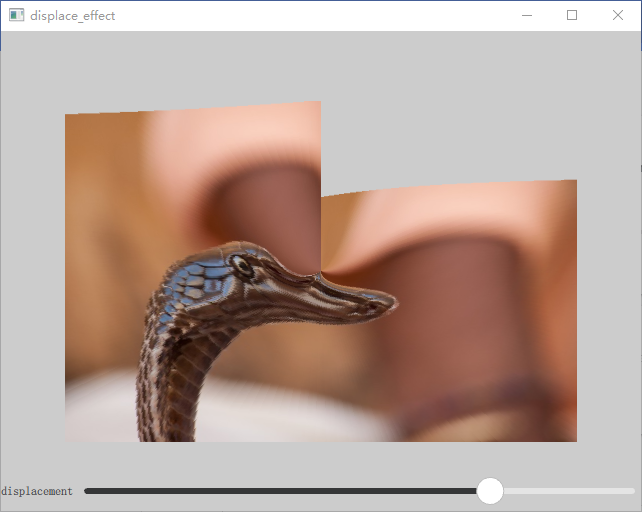
\includegraphics[width=0.95\textwidth]{../chapter06/displace_effect/the_app.png} %图片路径
\caption{Displace} %标题
\label{p000029} %索引
\end{figure}
%end图片


%\begin{spacing}{1.0}
\refstepcounter{filesourcenumber}\label{f000063}    %增加源代码编号
\FloatBarrier                                  %强制完成浮动体布局
\begin{thebookfilesourceone}[escapeinside={(*@}{@*)},
caption=GoodLuck,
title=\filesourcenumbernameone \thefilesourcenumber
]
/*displace_effect/main.qml*/
import QtQuick 2.9
import QtGraphicalEffects 1.12

Rectangle {
    id : idRoot
    width: 640;
    height: 480;
    color: Qt.rgba(0.8,0.8,0.8,1);

    Image{
        width: parent.width * 0.8;
        height: parent.height * 0.8;
        anchors.centerIn: parent
        source: "image.jpg"
        visible: false
        fillMode: Image.PreserveAspectFit
        id : idImage
    }

    ConicalGradient {
        anchors.fill: idImage
        source: idImage
        angle: 0.0
        gradient: Gradient {
            GradientStop { position: 0.0; color: "red" }
            GradientStop { position: 1.0; color: "green" }
        }
        visible: false
        id : idRedGreenDisplacement
    }

    Displace{
        anchors.fill: idImage
        source: idImage
        displacementSource: idRedGreenDisplacement
        displacement : thisControl.displacementItem.value
    }

    DisplaceControl{
        id : thisControl
    }

}(*@\marginpar[\hfill\setlength\fboxsep{2pt}\fbox{\footnotesize{\kaishu\parbox{1em}{\setlength{\baselineskip}{2pt}\filesourcenumbernameone}}\footnotesize{\thefilesourcenumber}}]{\setlength\fboxsep{2pt}\fbox{\footnotesize{\kaishu\parbox{1em}{\setlength{\baselineskip}{2pt}\filesourcenumbernameone}}\footnotesize{\thefilesourcenumber}}}@*)\end{thebookfilesourceone}          %抄录环境
\addtocounter{lstlisting}{-1}   %sub lstlisting counter ...
%\end{spacing}


未完待续






%使用XeLaTeX编译
%版权所有,翻版必究
%本文件由程序自动生成,任何修改将被覆盖
%2019 年 01 月 23 日





%使用XeLaTeX编译
%版权所有,翻版必究
%本文件由程序自动生成,任何修改将被覆盖
%2019 年 01 月 23 日




\FloatBarrier
\section{
DropShadow
}\label{c000015s000014}


%begin图片
\begin{figure}[htb] %浮动体 here and top ...
%there must use marginnote ...
\marginnote{\setlength\fboxsep{2pt}\fbox{\footnotesize{\kaishu\figurename\,}\footnotesize{\ref{p000030}}}}\centering %中心对齐
\setlength\fboxsep{0pt}\fcolorbox[rgb]{0,0,0}{0.97,0.98,0.99}{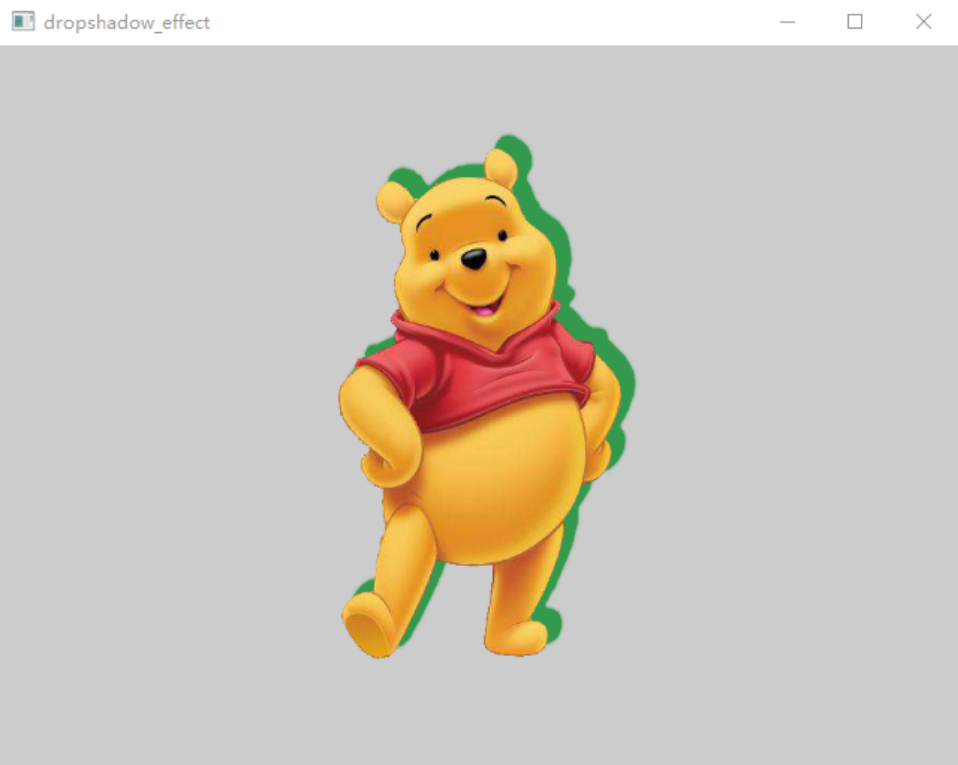
\includegraphics[width=0.95\textwidth]{the_book_image/p000030.pdf}} %图片路径
\caption{DropShadow} %标题
\label{p000030} %索引
\end{figure}
%end图片


%\begin{spacing}{1.0}
\refstepcounter{filesourcenumber}\label{f000064}    %增加源代码编号
\FloatBarrier                                  %强制完成浮动体布局
\begin{thebookfilesourceone}[escapeinside={(*@}{@*)},
caption=GoodLuck,
title=\filesourcenumbernameone \thefilesourcenumber
]
/*dropshadow_effect/main.qml*/
import QtQuick 2.9
import QtGraphicalEffects 1.12

Rectangle {
    id : idRoot
    width: 640;
    height: 480;
    color: Qt.rgba(0.8,0.8,0.8,1);

    Image{
        width: parent.width * 0.8;
        height: parent.height * 0.8;
        anchors.centerIn: parent
        source: "image"
        visible: false
        fillMode: Image.PreserveAspectFit
        id : idImage
    }

    DropShadow{
        color: Qt.rgba(0.2,0.6,0.3,1)
        horizontalOffset: 8
        verticalOffset: -8
        radius: 8
        samples: 36
        source: idImage
        spread: 0.5
        anchors.fill: idImage
    }

}(*@\marginpar[\hfill\setlength\fboxsep{2pt}\fbox{\footnotesize{\kaishu\parbox{1em}{\setlength{\baselineskip}{2pt}\filesourcenumbernameone}}\footnotesize{\thefilesourcenumber}}]{\setlength\fboxsep{2pt}\fbox{\footnotesize{\kaishu\parbox{1em}{\setlength{\baselineskip}{2pt}\filesourcenumbernameone}}\footnotesize{\thefilesourcenumber}}}@*)\end{thebookfilesourceone}          %抄录环境
\addtocounter{lstlisting}{-1}   %sub lstlisting counter ...
%\end{spacing}


未完待续






%使用XeLaTeX编译
%版权所有,翻版必究
%本文件由程序自动生成,任何修改将被覆盖
%2019 年 01 月 23 日





%使用XeLaTeX编译
%版权所有,翻版必究
%本文件由程序自动生成,任何修改将被覆盖
%2019 年 01 月 23 日




\FloatBarrier
\section{
InnerShadow
}\label{c000015s000015}


%begin图片
\begin{figure}[htb] %浮动体 here and top ...
%there must use marginnote not use marginnote ...
\marginnote{\setlength\fboxsep{2pt}\fbox{\footnotesize{\kaishu\figurename\,}\footnotesize{\ref{p000031}}}}\centering %中心对齐
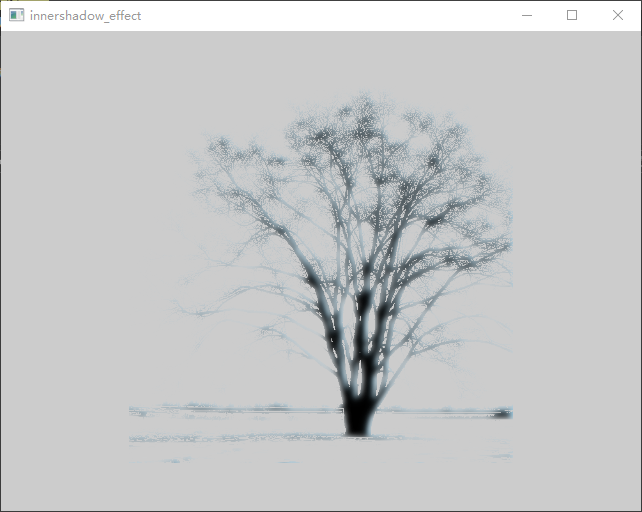
\includegraphics[width=0.95\textwidth]{../chapter06/innershadow_effect/the_app.png} %图片路径
\caption{InnerShadow} %标题
\label{p000031} %索引
\end{figure}
%end图片


%\begin{spacing}{1.0}
\refstepcounter{filesourcenumber}\label{f000065}    %增加源代码编号
\FloatBarrier                                  %强制完成浮动体布局
\begin{thebookfilesourceone}[escapeinside={(*@}{@*)},
caption=GoodLuck,
title=\filesourcenumbernameone \thefilesourcenumber
]
/*innershadow_effect/main.qml*/
import QtQuick 2.9
import QtGraphicalEffects 1.12

Rectangle {
    id : idRoot
    width: 640;
    height: 480;
    color: Qt.rgba(0.8,0.8,0.8,1);

    Image{
        width: parent.width * 0.8;
        height: parent.height * 0.8;
        anchors.centerIn: parent
        source: "image"
        visible: false
        fillMode: Image.PreserveAspectFit
        id : idImage
    }

    InnerShadow{
        anchors.fill: idImage
        source: idImage
        radius: 8
        samples: 16
        horizontalOffset: -3
        verticalOffset: 3
        color: Qt.rgba( 0.6,0.8,0.9,1 );
    }

}(*@\marginpar[\hfill\setlength\fboxsep{2pt}\fbox{\footnotesize{\kaishu\parbox{1em}{\setlength{\baselineskip}{2pt}\filesourcenumbernameone}}\footnotesize{\thefilesourcenumber}}]{\setlength\fboxsep{2pt}\fbox{\footnotesize{\kaishu\parbox{1em}{\setlength{\baselineskip}{2pt}\filesourcenumbernameone}}\footnotesize{\thefilesourcenumber}}}@*)\end{thebookfilesourceone}          %抄录环境
\addtocounter{lstlisting}{-1}   %sub lstlisting counter ...
%\end{spacing}


未完待续






%使用XeLaTeX编译
%版权所有,翻版必究
%本文件由程序自动生成,任何修改将被覆盖
%2019 年 01 月 23 日





%使用XeLaTeX编译
%版权所有,翻版必究
%本文件由程序自动生成,任何修改将被覆盖
%2019 年 01 月 23 日




\FloatBarrier
\section{
FastBlur
}\label{c000015s000016}


%begin图片
\begin{figure}[htb] %浮动体 here and top ...
%there must use marginnote ...
\marginnote{\setlength\fboxsep{2pt}\fbox{\footnotesize{\kaishu\figurename\,}\footnotesize{\ref{p000032}}}}\centering %中心对齐
\setlength\fboxsep{0pt}\fcolorbox[rgb]{0,0,0}{0.97,0.98,0.99}{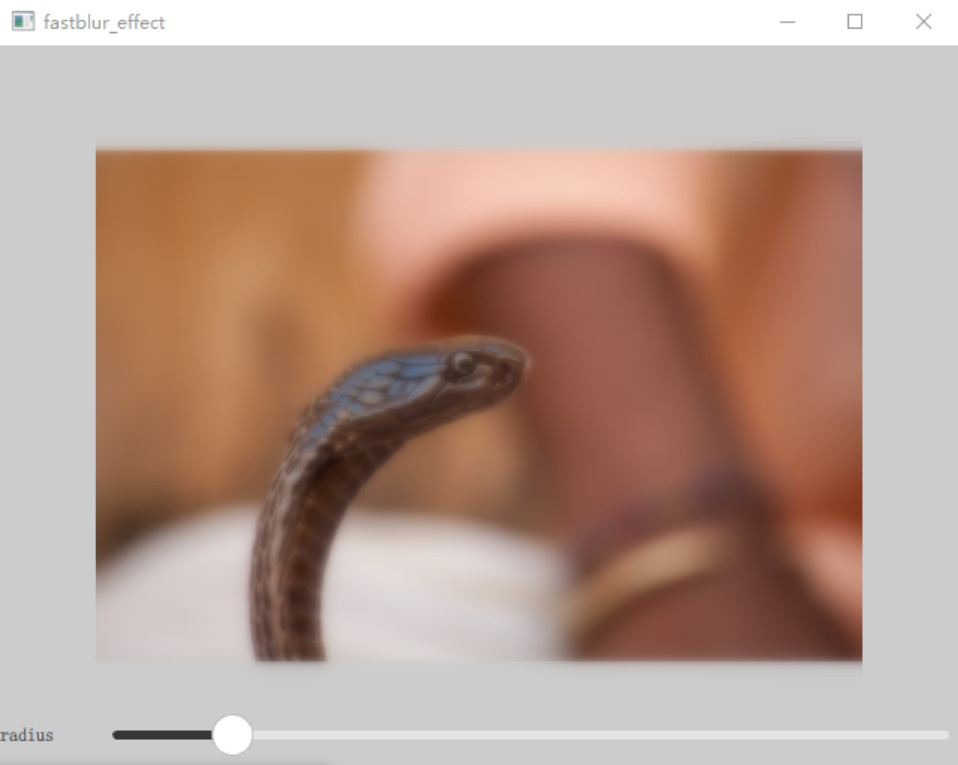
\includegraphics[width=0.95\textwidth]{the_book_image/p000032.pdf}} %图片路径
\caption{FastBlur} %标题
\label{p000032} %索引
\end{figure}
%end图片


%\begin{spacing}{1.0}
\refstepcounter{filesourcenumber}\label{f000066}    %增加源代码编号
\FloatBarrier                                  %强制完成浮动体布局
\begin{thebookfilesourceone}[escapeinside={(*@}{@*)},
caption=GoodLuck,
title=\filesourcenumbernameone \thefilesourcenumber
]
/*fastblur_effect/main.qml*/
import QtQuick 2.9
import QtGraphicalEffects 1.12

Rectangle {
    id : idRoot
    width: 640;
    height: 480;
    color: Qt.rgba(0.8,0.8,0.8,1);

    Image{
        width: parent.width * 0.8;
        height: parent.height * 0.8;
        anchors.centerIn: parent
        source: "image"
        visible: false
        fillMode: Image.PreserveAspectFit
        id : idImage
    }

    FastBlur{
        anchors.fill: idImage
        source: idImage
        radius: thisControl.radiusItem.value
    }

    FastBlurControl{
        id : thisControl
    }

}(*@\marginpar[\hfill\setlength\fboxsep{2pt}\fbox{\footnotesize{\kaishu\parbox{1em}{\setlength{\baselineskip}{2pt}\filesourcenumbernameone}}\footnotesize{\thefilesourcenumber}}]{\setlength\fboxsep{2pt}\fbox{\footnotesize{\kaishu\parbox{1em}{\setlength{\baselineskip}{2pt}\filesourcenumbernameone}}\footnotesize{\thefilesourcenumber}}}@*)\end{thebookfilesourceone}          %抄录环境
\addtocounter{lstlisting}{-1}   %sub lstlisting counter ...
%\end{spacing}


未完待续


% ______all_key_words
% the_book_chapter the_book_subsection the_book_subsubsection
% the_book_section the_book_image the_book_table
% the_book_file the_book_tree_file the_book_command_file
% littlelongworld tabbing ref
% figurename tablename filesourcenumbernameone
% treeindexnumbernameone commandnumbernameone footnote 
% item itemize comment textbullet
% \hspace*{\parindent}







%使用XeLaTeX编译
%版权所有,翻版必究
%本文件由程序自动生成,任何修改将被覆盖
%2019 年 01 月 23 日





%使用XeLaTeX编译
%版权所有,翻版必究
%本文件由程序自动生成,任何修改将被覆盖
%2019 年 01 月 23 日




\FloatBarrier
\section{
GaussianBlur
}\label{c000015s000017}


%begin图片
\begin{figure}[htb] %浮动体 here and top ...
%there must use marginnote ...
\marginnote{\setlength\fboxsep{2pt}\fbox{\footnotesize{\kaishu\figurename\,}\footnotesize{\ref{p000033}}}}\centering %中心对齐
\setlength\fboxsep{0pt}\fcolorbox[rgb]{0,0,0}{0.97,0.98,0.99}{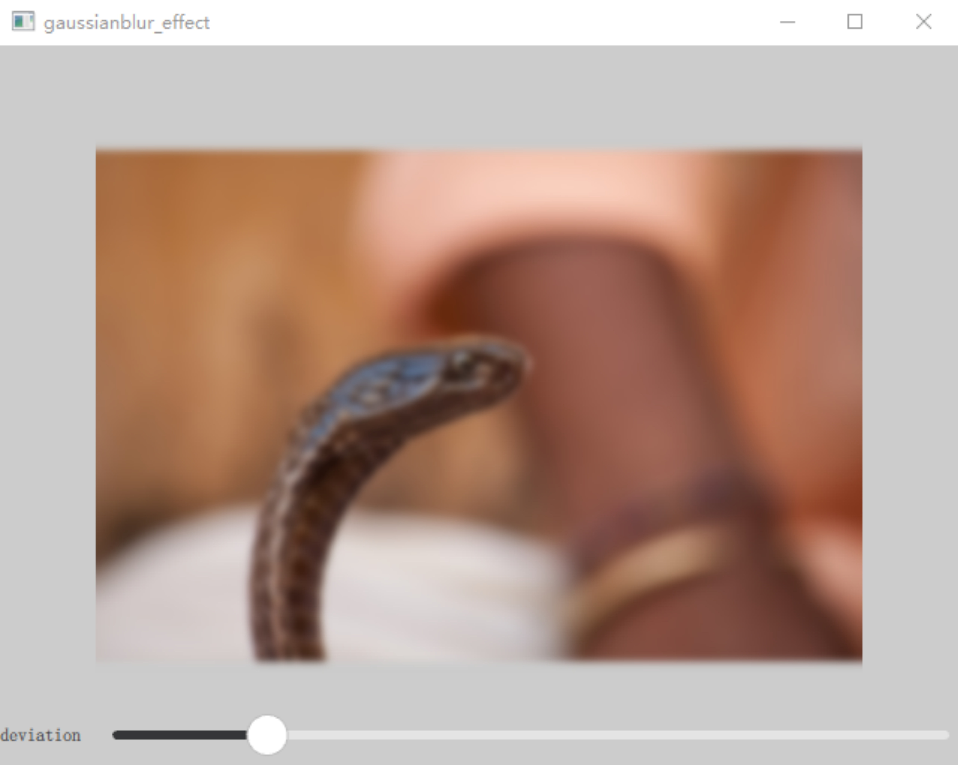
\includegraphics[width=0.95\textwidth]{the_book_image/p000033.pdf}} %图片路径
\caption{GaussianBlur} %标题
\label{p000033} %索引
\end{figure}
%end图片


%\begin{spacing}{1.0}
\refstepcounter{filesourcenumber}\label{f000067}    %增加源代码编号
\FloatBarrier                                  %强制完成浮动体布局
\begin{thebookfilesourceone}[escapeinside={(*@}{@*)},
caption=GoodLuck,
title=\filesourcenumbernameone \thefilesourcenumber
]
/*gaussianblur_effect/main.qml*/
import QtQuick 2.9
import QtGraphicalEffects 1.12

Rectangle {
    id : idRoot
    width: 640;
    height: 480;
    color: Qt.rgba(0.8,0.8,0.8,1);

    Image{
        width: parent.width * 0.8;
        height: parent.height * 0.8;
        anchors.centerIn: parent
        source: "image"
        visible: false
        fillMode: Image.PreserveAspectFit
        id : idImage
    }

    GaussianBlur{
        anchors.fill: idImage
        source: idImage
        radius: 8
        samples: 16
        deviation: idThisControl.deviationItem.value
    }

    GaussianBlurControl{
        id : idThisControl
    }

}(*@\marginpar[\hfill\setlength\fboxsep{2pt}\fbox{\footnotesize{\kaishu\parbox{1em}{\setlength{\baselineskip}{2pt}\filesourcenumbernameone}}\footnotesize{\thefilesourcenumber}}]{\setlength\fboxsep{2pt}\fbox{\footnotesize{\kaishu\parbox{1em}{\setlength{\baselineskip}{2pt}\filesourcenumbernameone}}\footnotesize{\thefilesourcenumber}}}@*)\end{thebookfilesourceone}          %抄录环境
\addtocounter{lstlisting}{-1}   %sub lstlisting counter ...
%\end{spacing}


未完待续






%使用XeLaTeX编译
%版权所有,翻版必究
%本文件由程序自动生成,任何修改将被覆盖
%2019 年 01 月 23 日





%使用XeLaTeX编译
%版权所有,翻版必究
%本文件由程序自动生成,任何修改将被覆盖
%2019 年 01 月 23 日




\FloatBarrier
\section{
MaskedBlur
}\label{c000015s000018}


%begin图片
\begin{figure}[htb] %浮动体 here and top ...
%there must use marginnote ...
\marginnote{\setlength\fboxsep{2pt}\fbox{\footnotesize{\kaishu\figurename\,}\footnotesize{\ref{p000034}}}}\centering %中心对齐
\setlength\fboxsep{0pt}\fcolorbox[rgb]{0,0,0}{0,0,0}{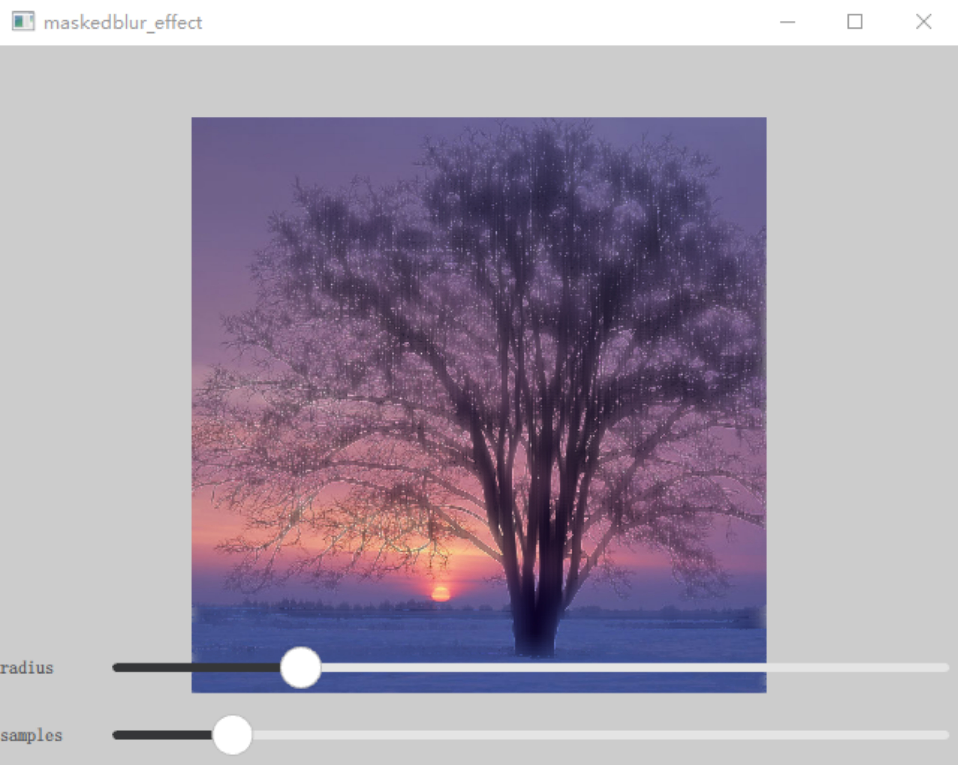
\includegraphics[width=0.95\textwidth]{the_book_image/p000034.pdf}} %图片路径
\caption{MaskedBlur} %标题
\label{p000034} %索引
\end{figure}
%end图片


%\begin{spacing}{1.0}
\refstepcounter{filesourcenumber}\label{f000068}    %增加源代码编号
\FloatBarrier                                  %强制完成浮动体布局
\begin{thebookfilesourceone}[escapeinside={(*@}{@*)},
caption=GoodLuck,
title=\filesourcenumbernameone \thefilesourcenumber
]
/*maskedblur_effect/main.qml*/
import QtQuick 2.9
import QtGraphicalEffects 1.12

Rectangle {
    id : idRoot
    width: 640;
    height: 480;
    color: Qt.rgba(0.8,0.8,0.8,1);

    Image{
        width: parent.width * 0.8;
        height: parent.height * 0.8;
        anchors.centerIn: parent
        source: "image.png"
        visible: false
        fillMode: Image.PreserveAspectFit
        id : idMask
    }

    Image{
        width: parent.width * 0.8;
        height: parent.height * 0.8;
        anchors.centerIn: parent
        source: "image.jpg"
        visible: false
        fillMode: Image.PreserveAspectFit
        id : idImage
    }

    MaskedBlur{
        source: idImage
        maskSource: idMask
        anchors.fill: idImage
        radius: idThisControl.radiusItem.value
        samples: idThisControl.samplesItem.value
    }

    MaskedBlurControl{
        id : idThisControl
    }

}(*@\marginpar[\hfill\setlength\fboxsep{2pt}\fbox{\footnotesize{\kaishu\parbox{1em}{\setlength{\baselineskip}{2pt}\filesourcenumbernameone}}\footnotesize{\thefilesourcenumber}}]{\setlength\fboxsep{2pt}\fbox{\footnotesize{\kaishu\parbox{1em}{\setlength{\baselineskip}{2pt}\filesourcenumbernameone}}\footnotesize{\thefilesourcenumber}}}@*)\end{thebookfilesourceone}          %抄录环境
\addtocounter{lstlisting}{-1}   %sub lstlisting counter ...
%\end{spacing}


未完待续






%使用XeLaTeX编译
%版权所有,翻版必究
%本文件由程序自动生成,任何修改将被覆盖
%2019 年 01 月 23 日





%使用XeLaTeX编译
%版权所有,翻版必究
%本文件由程序自动生成,任何修改将被覆盖
%2019 年 01 月 23 日




\FloatBarrier
\section{
RecursiveBlur
}\label{c000015s000019}


%begin图片
\begin{figure}[htb] %浮动体 here and top ...
%there must use marginnote ...
\marginnote{\setlength\fboxsep{2pt}\fbox{\footnotesize{\kaishu\figurename\,}\footnotesize{\ref{p000035}}}}\centering %中心对齐
\setlength\fboxsep{0pt}\fcolorbox[rgb]{0,0,0}{0.97,0.98,0.99}{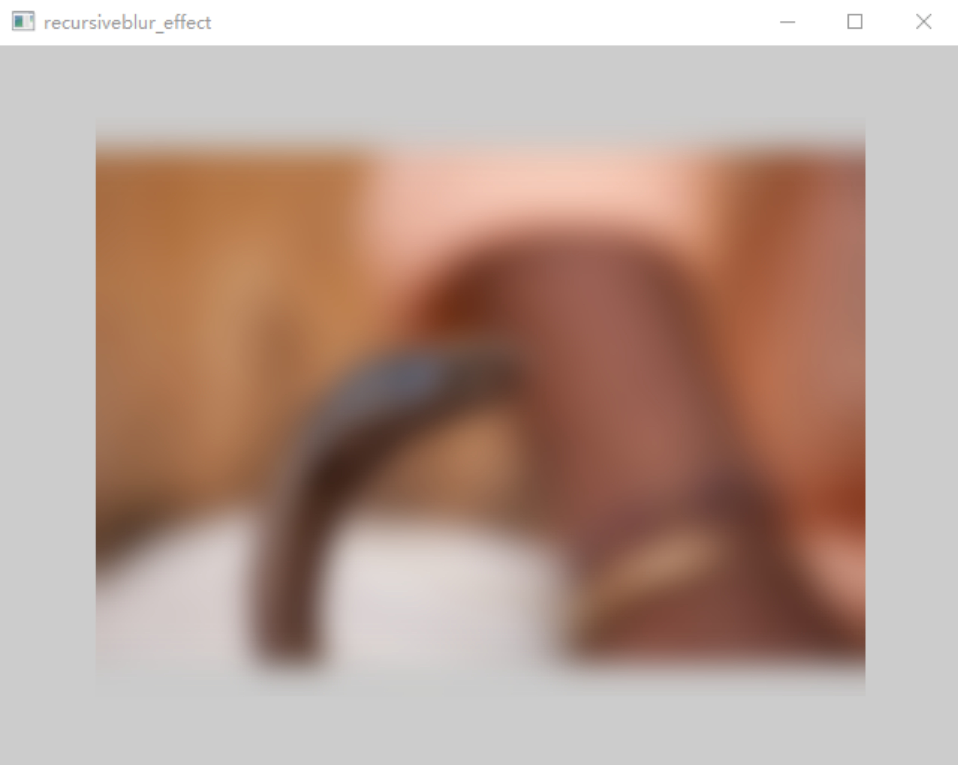
\includegraphics[width=0.95\textwidth]{the_book_image/p000035.pdf}} %图片路径
\caption{RecursiveBlur} %标题
\label{p000035} %索引
\end{figure}
%end图片


%\begin{spacing}{1.0}
\refstepcounter{filesourcenumber}\label{f000069}    %增加源代码编号
\FloatBarrier                                  %强制完成浮动体布局
\begin{thebookfilesourceone}[escapeinside={(*@}{@*)},
caption=GoodLuck,
title=\filesourcenumbernameone \thefilesourcenumber
]
/*recursiveblur_effect/main.qml*/
import QtQuick 2.9
import QtGraphicalEffects 1.12

Rectangle {
    id : idRoot
    width: 640;
    height: 480;
    color: Qt.rgba(0.8,0.8,0.8,1);

    Image{
        width: parent.width * 0.8;
        height: parent.height * 0.8;
        anchors.centerIn: parent
        source: "image.jpg"
        visible: false
        fillMode: Image.PreserveAspectFit
        id : idImage
    }

    RecursiveBlur{
        anchors.fill: idImage
        source: idImage
        loops: 8
        radius: 8
    }
}(*@\marginpar[\hfill\setlength\fboxsep{2pt}\fbox{\footnotesize{\kaishu\parbox{1em}{\setlength{\baselineskip}{2pt}\filesourcenumbernameone}}\footnotesize{\thefilesourcenumber}}]{\setlength\fboxsep{2pt}\fbox{\footnotesize{\kaishu\parbox{1em}{\setlength{\baselineskip}{2pt}\filesourcenumbernameone}}\footnotesize{\thefilesourcenumber}}}@*)\end{thebookfilesourceone}          %抄录环境
\addtocounter{lstlisting}{-1}   %sub lstlisting counter ...
%\end{spacing}


未完待续






%使用XeLaTeX编译
%版权所有,翻版必究
%本文件由程序自动生成,任何修改将被覆盖
%2019 年 01 月 23 日





%使用XeLaTeX编译
%版权所有,翻版必究
%本文件由程序自动生成,任何修改将被覆盖
%2019 年 01 月 23 日




\FloatBarrier
\section{
DirectionalBlur
}\label{c000015s000020}


%begin图片
\begin{figure}[htb] %浮动体 here and top ...
%there must use marginnote ...
\marginnote{\setlength\fboxsep{2pt}\fbox{\footnotesize{\kaishu\figurename\,}\footnotesize{\ref{p000036}}}}\centering %中心对齐
\setlength\fboxsep{0pt}\fbox{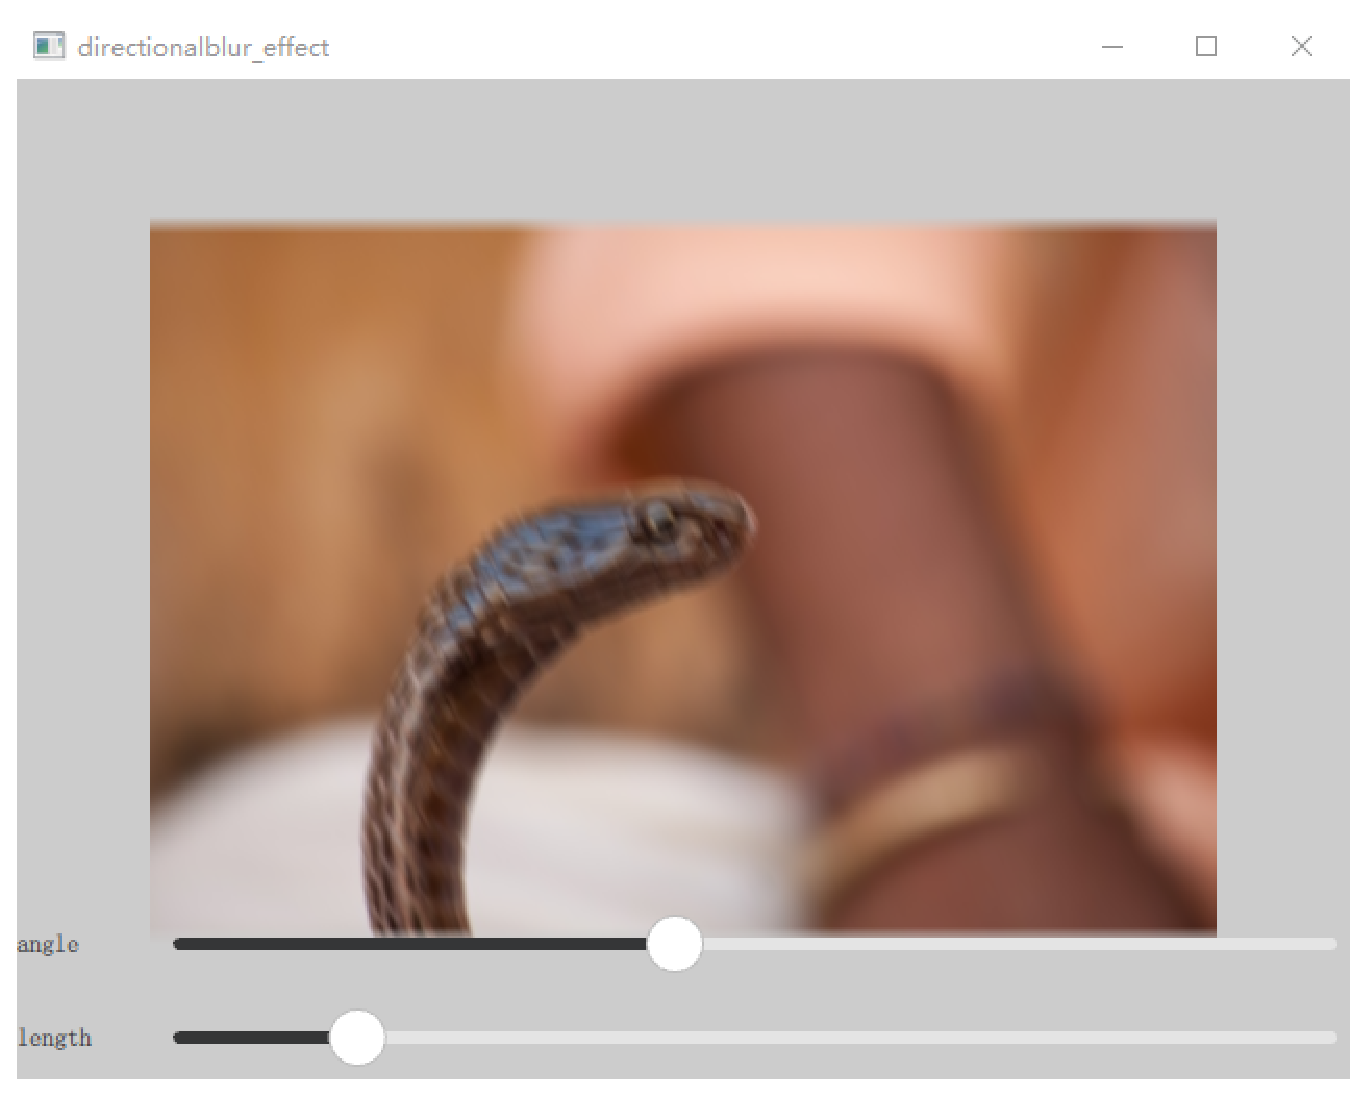
\includegraphics[width=0.95\textwidth]{the_book_image/p000036.eps}} %图片路径
\caption{DirectionalBlur} %标题
\label{p000036} %索引
\end{figure}
%end图片


%\begin{spacing}{1.0}
\refstepcounter{filesourcenumber}\label{f000070}    %增加源代码编号
\FloatBarrier                                  %强制完成浮动体布局
\begin{thebookfilesourceone}[escapeinside={(*@}{@*)},
caption=GoodLuck,
title=\filesourcenumbernameone \thefilesourcenumber
]
/*directionalblur_effect/main.qml*/
import QtQuick 2.9
import QtGraphicalEffects 1.12

Rectangle {
    id : idRoot
    width: 640;
    height: 480;
    color: Qt.rgba(0.8,0.8,0.8,1);

    Image{
        width: parent.width * 0.8;
        height: parent.height * 0.8;
        anchors.centerIn: parent
        source: "image.jpg"
        visible: false
        fillMode: Image.PreserveAspectFit
        id : idImage
    }

    DirectionalBlur{
        anchors.fill: idImage
        source: idImage
        samples: 64
        length: idThisControl.lengthItem.value
        angle: idThisControl.angleItem.value
        transparentBorder : false
        id:idEffect
    }

    DirectionalblurControl{
        id : idThisControl
        lengthItem.to: idEffect.samples
    }

}(*@\marginpar[\hfill\setlength\fboxsep{2pt}\fbox{\footnotesize{\kaishu\parbox{1em}{\setlength{\baselineskip}{2pt}\filesourcenumbernameone}}\footnotesize{\thefilesourcenumber}}]{\setlength\fboxsep{2pt}\fbox{\footnotesize{\kaishu\parbox{1em}{\setlength{\baselineskip}{2pt}\filesourcenumbernameone}}\footnotesize{\thefilesourcenumber}}}@*)\end{thebookfilesourceone}          %抄录环境
\addtocounter{lstlisting}{-1}   %sub lstlisting counter ...
%\end{spacing}


未完待续






%使用XeLaTeX编译
%版权所有,翻版必究
%本文件由程序自动生成,任何修改将被覆盖
%2019 年 01 月 23 日





%使用XeLaTeX编译
%版权所有,翻版必究
%本文件由程序自动生成,任何修改将被覆盖
%2019 年 01 月 23 日




\FloatBarrier
\section{
RadialBlur
}\label{c000015s000021}


%begin图片
\begin{figure}[htb] %浮动体 here and top ...
%there must use marginnote ...
\marginnote{\setlength\fboxsep{2pt}\fbox{\footnotesize{\kaishu\figurename\,}\footnotesize{\ref{p000037}}}}\centering %中心对齐
\setlength\fboxsep{0pt}\fcolorbox[rgb]{0,0,0}{0.97,0.98,0.99}{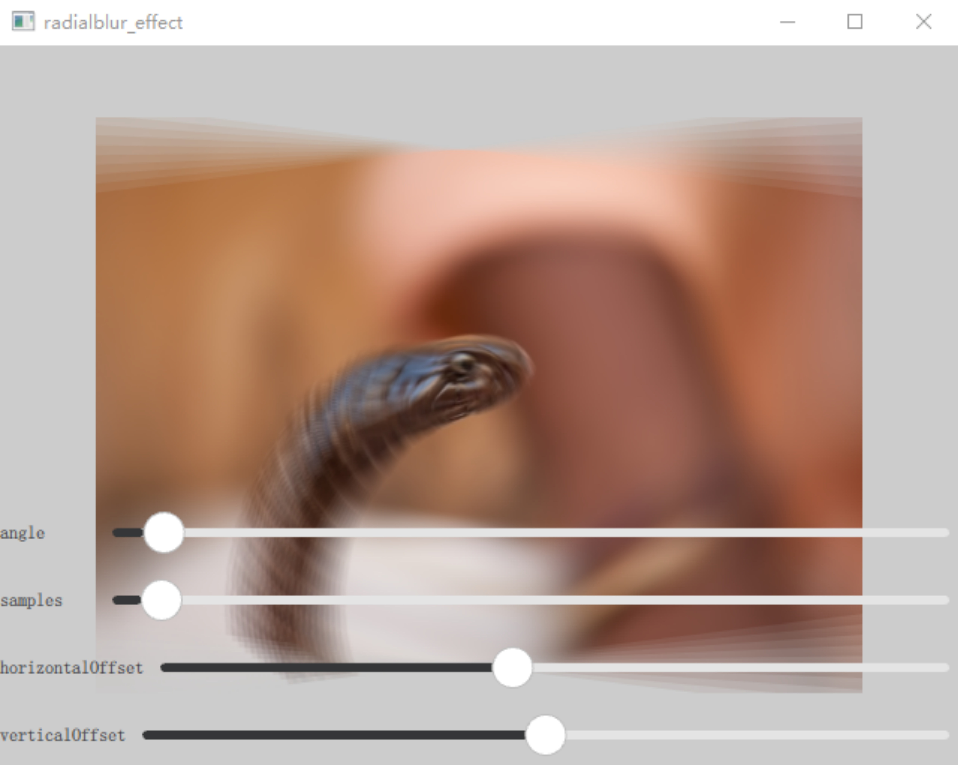
\includegraphics[width=0.95\textwidth]{the_book_image/p000037.pdf}} %图片路径
\caption{RadialBlur} %标题
\label{p000037} %索引
\end{figure}
%end图片


%\begin{spacing}{1.0}
\refstepcounter{filesourcenumber}\label{f000071}    %增加源代码编号
\FloatBarrier                                  %强制完成浮动体布局
\begin{thebookfilesourceone}[escapeinside={(*@}{@*)},
caption=GoodLuck,
title=\filesourcenumbernameone \thefilesourcenumber
]
/*radialblur_effect/main.qml*/
import QtQuick 2.9
import QtGraphicalEffects 1.12

Rectangle {
    id : idRoot
    width: 640;
    height: 480;
    color: Qt.rgba(0.8,0.8,0.8,1);

    Image{
        width: parent.width * 0.8;
        height: parent.height * 0.8;
        anchors.centerIn: parent
        source: "image.jpg"
        visible: false
        fillMode: Image.PreserveAspectFit
        id : idImage
    }

    RadialBlur{
        anchors.fill: idImage
        source: idImage
        angle: thisControl.angleItem.value
        samples: thisControl.samplesItem.value
        verticalOffset:
            thisControl.verticalOffsetItem.value
        horizontalOffset:
            thisControl.horizontalOffsetItem.value
    }

    RadialBlurControl{
        id : thisControl
    }

}(*@\marginpar[\hfill\setlength\fboxsep{2pt}\fbox{\footnotesize{\kaishu\parbox{1em}{\setlength{\baselineskip}{2pt}\filesourcenumbernameone}}\footnotesize{\thefilesourcenumber}}]{\setlength\fboxsep{2pt}\fbox{\footnotesize{\kaishu\parbox{1em}{\setlength{\baselineskip}{2pt}\filesourcenumbernameone}}\footnotesize{\thefilesourcenumber}}}@*)\end{thebookfilesourceone}          %抄录环境
\addtocounter{lstlisting}{-1}   %sub lstlisting counter ...
%\end{spacing}


未完待续


% ______all_key_words
% the_book_chapter the_book_subsection the_book_subsubsection
% the_book_section the_book_image the_book_table
% the_book_file the_book_tree_file the_book_command_file
% littlelongworld tabbing ref
% figurename tablename filesourcenumbernameone
% treeindexnumbernameone commandnumbernameone footnote
% item itemize comment textbullet
% \hspace*{\parindent}







%使用XeLaTeX编译
%版权所有,翻版必究
%本文件由程序自动生成,任何修改将被覆盖
%2019 年 01 月 23 日





%使用XeLaTeX编译
%版权所有,翻版必究
%本文件由程序自动生成,任何修改将被覆盖
%2019 年 01 月 23 日




\FloatBarrier
\section{
ZoomBlur
}\label{c000015s000022}


%begin图片
\begin{figure}[htb] %浮动体 here and top ...
%there must use marginnote ...
\marginnote{\setlength\fboxsep{2pt}\fbox{\footnotesize{\kaishu\figurename\,}\footnotesize{\ref{p000038}}}}\centering %中心对齐
\setlength\fboxsep{0pt}\fcolorbox[rgb]{0,0,0}{0,0,0}{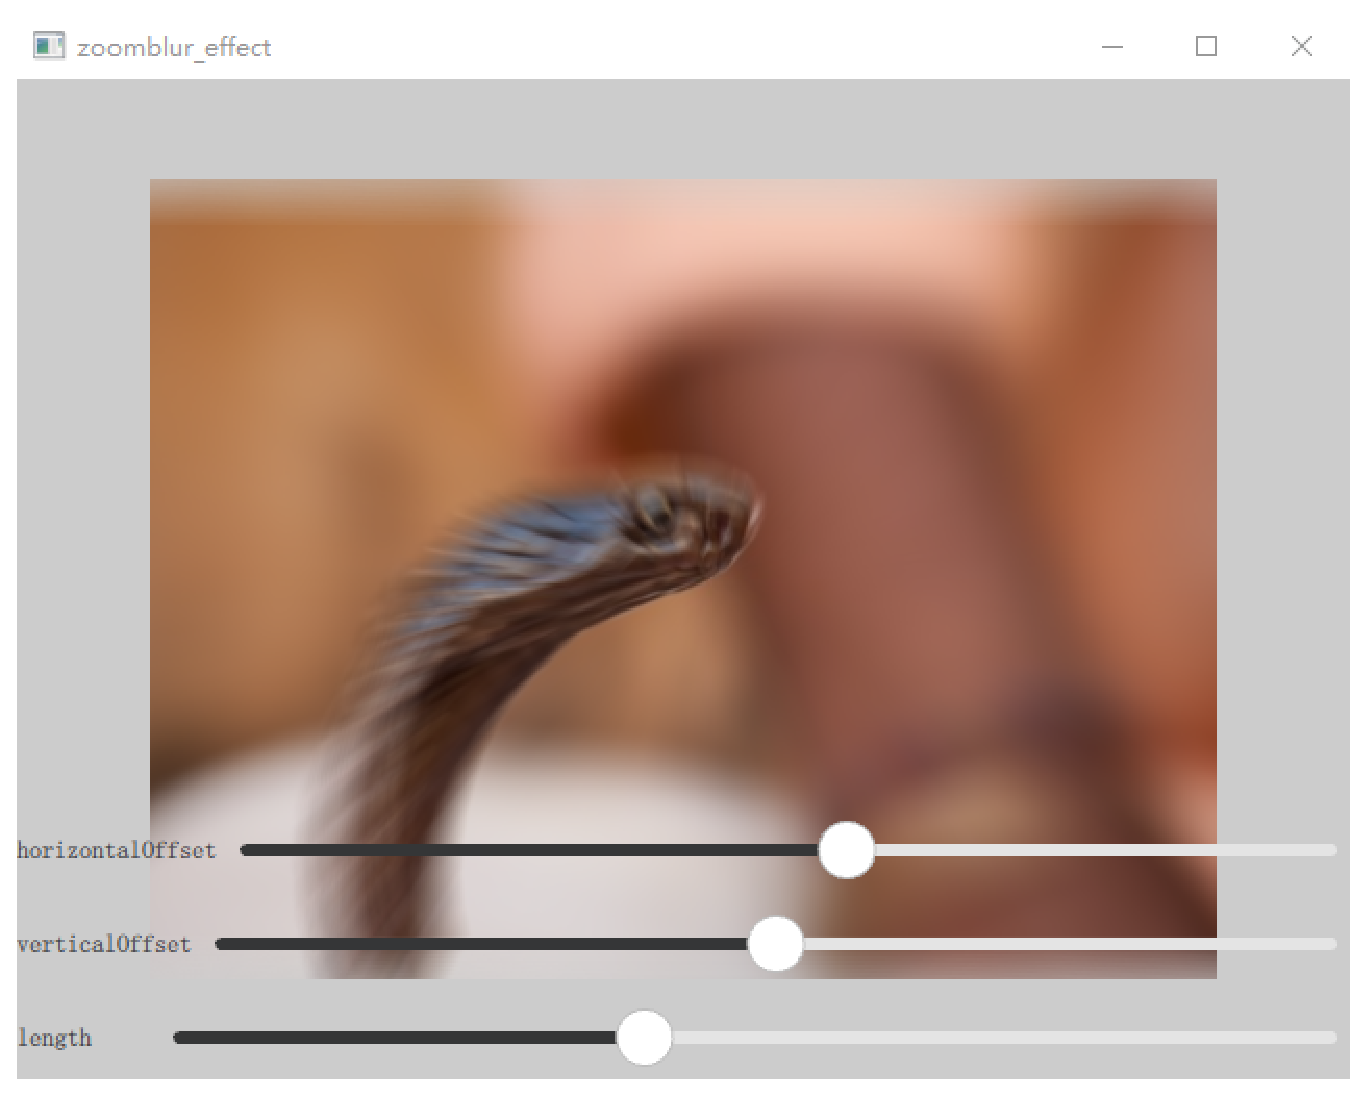
\includegraphics[width=0.95\textwidth]{the_book_image/p000038.eps}} %图片路径
\caption{ZoomBlur} %标题
\label{p000038} %索引
\end{figure}
%end图片


%\begin{spacing}{1.0}
\refstepcounter{filesourcenumber}\label{f000072}    %增加源代码编号
\FloatBarrier                                  %强制完成浮动体布局
\begin{thebookfilesourceone}[escapeinside={(*@}{@*)},
caption=GoodLuck,
title=\filesourcenumbernameone \thefilesourcenumber
]
/*zoomblur_effect/main.qml*/
import QtQuick 2.9
import QtGraphicalEffects 1.12

Rectangle {
    id : idRoot
    width: 640;
    height: 480;
    color: Qt.rgba(0.8,0.8,0.8,1);

    Image{
        width: parent.width * 0.8;
        height: parent.height * 0.8;
        anchors.centerIn: parent
        source: "image"
        visible: false
        fillMode: Image.PreserveAspectFit
        id : idImage
    }

    ZoomBlur {
        anchors.fill: idImage
        source: idImage
        samples: 24
        length:
            idThisControl.lengthItem.value
        verticalOffset:
            idThisControl.verticalOffsetItem.value
        horizontalOffset :
            idThisControl.horizontalOffsetItem.value
    }

    ZoomBlurControl{
        id : idThisControl
    }

}(*@\marginpar[\hfill\setlength\fboxsep{2pt}\fbox{\footnotesize{\kaishu\parbox{1em}{\setlength{\baselineskip}{2pt}\filesourcenumbernameone}}\footnotesize{\thefilesourcenumber}}]{\setlength\fboxsep{2pt}\fbox{\footnotesize{\kaishu\parbox{1em}{\setlength{\baselineskip}{2pt}\filesourcenumbernameone}}\footnotesize{\thefilesourcenumber}}}@*)\end{thebookfilesourceone}          %抄录环境
\addtocounter{lstlisting}{-1}   %sub lstlisting counter ...
%\end{spacing}


未完待续






%使用XeLaTeX编译
%版权所有,翻版必究
%本文件由程序自动生成,任何修改将被覆盖
%2019 年 01 月 23 日





%使用XeLaTeX编译
%版权所有,翻版必究
%本文件由程序自动生成,任何修改将被覆盖
%2019 年 01 月 23 日




\FloatBarrier
\section{
Glow
}\label{c000015s000023}


%begin图片
\begin{figure}[htb] %浮动体 here and top ...
%there must use marginnote ...
\marginnote{\setlength\fboxsep{2pt}\fbox{\footnotesize{\kaishu\figurename\,}\footnotesize{\ref{p000039}}}}\centering %中心对齐
\setlength\fboxsep{0pt}\fbox{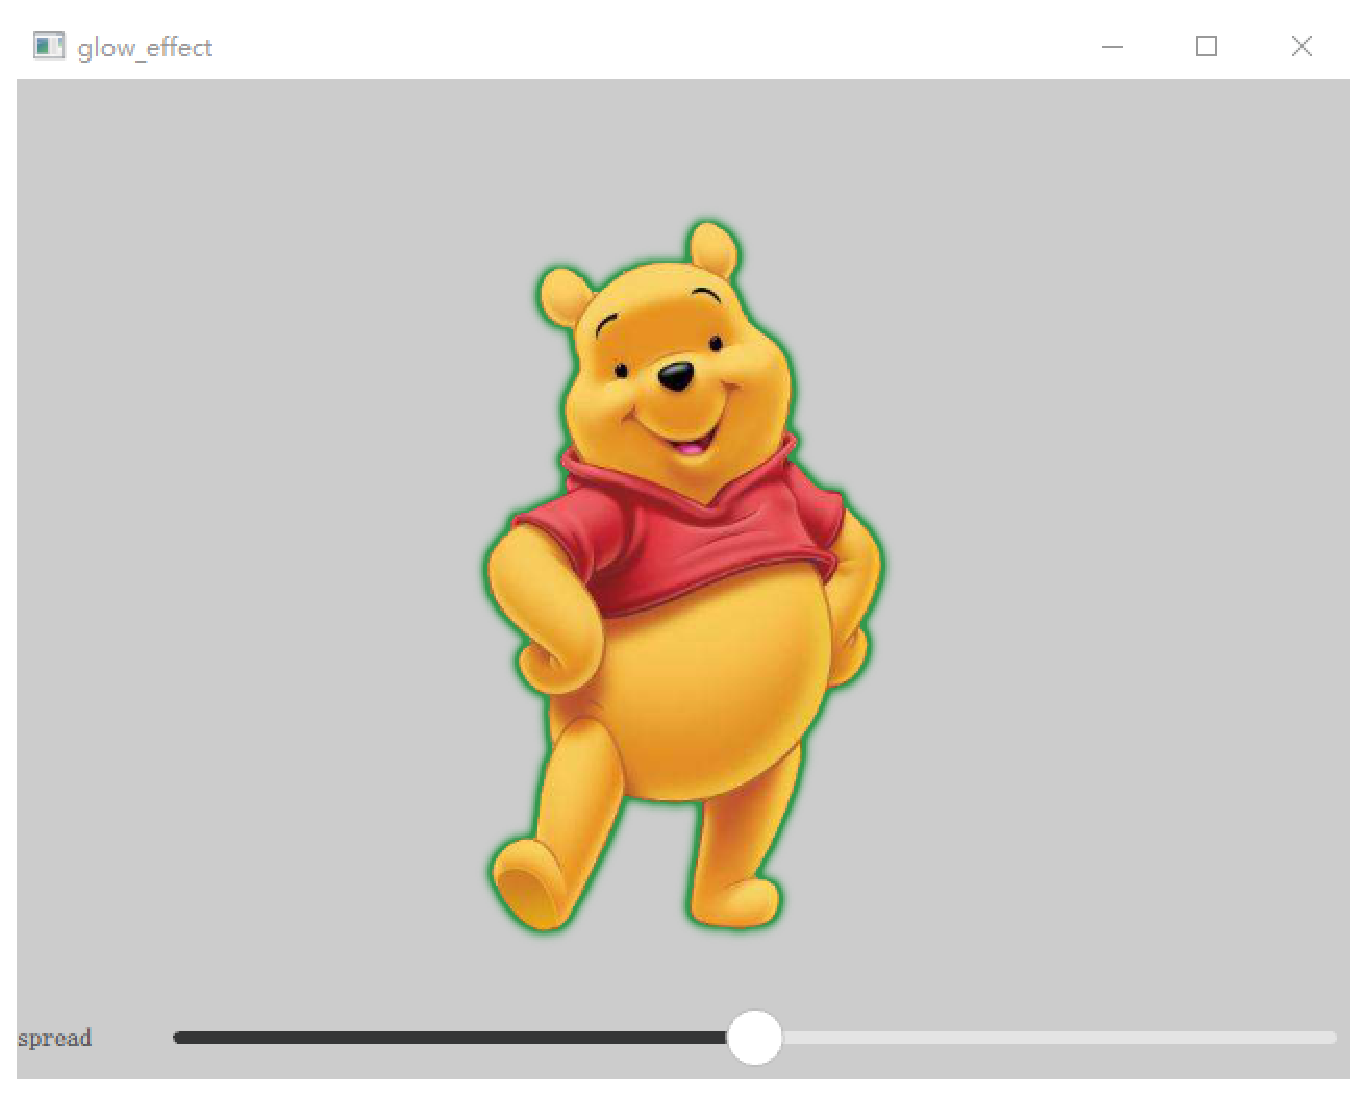
\includegraphics[width=0.95\textwidth]{the_book_image/p000039.eps}} %图片路径
\caption{Glow} %标题
\label{p000039} %索引
\end{figure}
%end图片


%\begin{spacing}{1.0}
\refstepcounter{filesourcenumber}\label{f000073}    %增加源代码编号
\FloatBarrier                                  %强制完成浮动体布局
\begin{thebookfilesourceone}[escapeinside={(*@}{@*)},
caption=GoodLuck,
title=\filesourcenumbernameone \thefilesourcenumber
]
/*glow_effect/main.qml*/
import QtQuick 2.9
import QtGraphicalEffects 1.12

Rectangle {
    id : idRoot
    width: 640;
    height: 480;
    color: Qt.rgba(0.8,0.8,0.8,1);

    Image{
        width: parent.width * 0.8;
        height: parent.height * 0.8;
        anchors.centerIn: parent
        source: "image"
        visible: false
        fillMode: Image.PreserveAspectFit
        id : idImage
    }

    Glow{
        color: Qt.rgba(0.2,0.6,0.3,1)
        radius: 8
        samples: 16
        spread: idThisControl.spreadItem.value
        anchors.fill: idImage
        source: idImage
    }

    GlowControl{
        id : idThisControl
    }

}(*@\marginpar[\hfill\setlength\fboxsep{2pt}\fbox{\footnotesize{\kaishu\parbox{1em}{\setlength{\baselineskip}{2pt}\filesourcenumbernameone}}\footnotesize{\thefilesourcenumber}}]{\setlength\fboxsep{2pt}\fbox{\footnotesize{\kaishu\parbox{1em}{\setlength{\baselineskip}{2pt}\filesourcenumbernameone}}\footnotesize{\thefilesourcenumber}}}@*)\end{thebookfilesourceone}          %抄录环境
\addtocounter{lstlisting}{-1}   %sub lstlisting counter ...
%\end{spacing}


未完待续






%使用XeLaTeX编译
%版权所有,翻版必究
%本文件由程序自动生成,任何修改将被覆盖
%2019 年 01 月 23 日





%使用XeLaTeX编译
%版权所有,翻版必究
%本文件由程序自动生成,任何修改将被覆盖
%2019 年 01 月 23 日




\FloatBarrier
\section{
RectangularGlow
}\label{c000015s000024}


%begin图片
\begin{figure}[htb] %浮动体 here and top ...
%there must use marginnote ...
\marginnote{\setlength\fboxsep{2pt}\fbox{\footnotesize{\kaishu\figurename\,}\footnotesize{\ref{p000040}}}}\centering %中心对齐
\setlength\fboxsep{0pt}\fcolorbox[rgb]{0,0,0}{0.97,0.98,0.99}{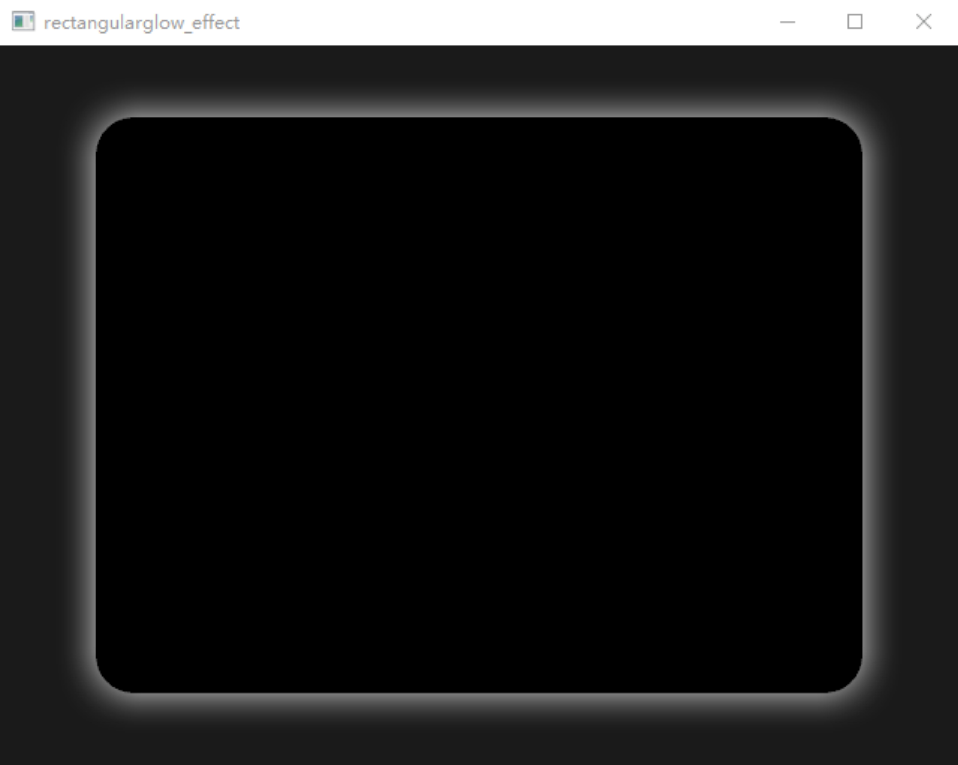
\includegraphics[width=0.95\textwidth]{the_book_image/p000040.pdf}} %图片路径
\caption{RectangularGlow} %标题
\label{p000040} %索引
\end{figure}
%end图片


%\begin{spacing}{1.0}
\refstepcounter{filesourcenumber}\label{f000074}    %增加源代码编号
\FloatBarrier                                  %强制完成浮动体布局
\begin{thebookfilesourceone}[escapeinside={(*@}{@*)},
caption=GoodLuck,
title=\filesourcenumbernameone \thefilesourcenumber
]
/*rectangularglow_effect/main.qml*/
import QtQuick 2.9
import QtGraphicalEffects 1.12

Rectangle {
    id : idRoot
    width: 640;
    height: 480;
    color: Qt.rgba(0.1,0.1,0.1,1);

    RectangularGlow {
        id: idEffect
        anchors.fill: idRect
        glowRadius: 10
        spread: 0.2
        color: "white"
        cornerRadius: glowRadius + idRect.radius
    }

    Rectangle {
        id: idRect
        color: "black"
        width: parent.width * 0.8
        height: parent.height * 0.8
        anchors.centerIn: parent
        radius: 25
    }

}(*@\marginpar[\hfill\setlength\fboxsep{2pt}\fbox{\footnotesize{\kaishu\parbox{1em}{\setlength{\baselineskip}{2pt}\filesourcenumbernameone}}\footnotesize{\thefilesourcenumber}}]{\setlength\fboxsep{2pt}\fbox{\footnotesize{\kaishu\parbox{1em}{\setlength{\baselineskip}{2pt}\filesourcenumbernameone}}\footnotesize{\thefilesourcenumber}}}@*)\end{thebookfilesourceone}          %抄录环境
\addtocounter{lstlisting}{-1}   %sub lstlisting counter ...
%\end{spacing}


未完待续


% ______all_key_words
% the_book_chapter the_book_subsection the_book_subsubsection
% the_book_section the_book_image the_book_table
% the_book_file the_book_tree_file the_book_command_file
% littlelongworld tabbing ref
% figurename tablename filesourcenumbernameone
% treeindexnumbernameone commandnumbernameone footnote
% item itemize comment textbullet
% \hspace*{\parindent}
% FloatBarrier







%使用XeLaTeX编译
%版权所有,翻版必究
%本文件由程序自动生成,任何修改将被覆盖
%2019 年 01 月 23 日





%使用XeLaTeX编译
%版权所有,翻版必究
%本文件由程序自动生成,任何修改将被覆盖
%2019 年 01 月 23 日




\FloatBarrier
\section{
OpacityMask
}\label{c000015s000025}


%begin图片
\begin{figure}[htb] %浮动体 here and top ...
%there must use marginnote ...
\marginnote{\setlength\fboxsep{2pt}\fbox{\footnotesize{\kaishu\figurename\,}\footnotesize{\ref{p000041}}}}\centering %中心对齐
\setlength\fboxsep{0pt}\fbox{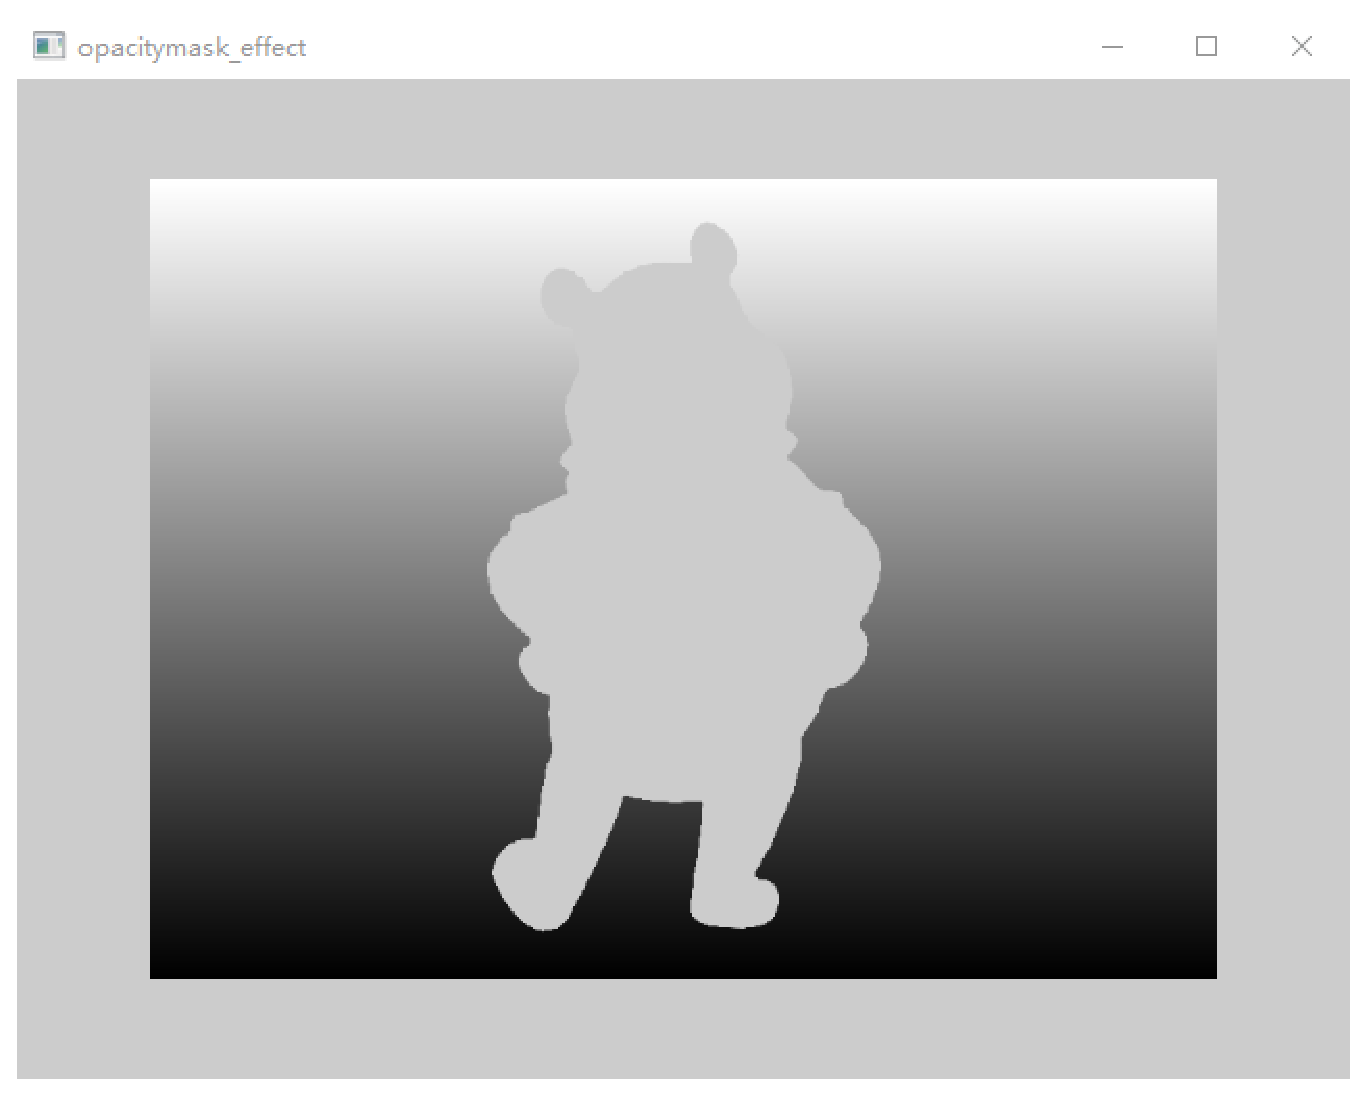
\includegraphics[width=0.95\textwidth]{the_book_image/p000041.eps}} %图片路径
\caption{OpacityMask} %标题
\label{p000041} %索引
\end{figure}
%end图片


%\begin{spacing}{1.0}
\refstepcounter{filesourcenumber}\label{f000075}    %增加源代码编号
\FloatBarrier                                  %强制完成浮动体布局
\begin{thebookfilesourceone}[escapeinside={(*@}{@*)},
caption=GoodLuck,
title=\filesourcenumbernameone \thefilesourcenumber
]
/*opacitymask_effect/main.qml*/
import QtQuick 2.9
import QtGraphicalEffects 1.12

Rectangle {
    id : idRoot
    width: 640;
    height: 480;
    color: Qt.rgba(0.8,0.8,0.8,1);

    Image{
        width: parent.width * 0.8;
        height: parent.height * 0.8;
        anchors.centerIn: parent
        source: "image"
        visible: false
        fillMode: Image.PreserveAspectFit
        id : idMask
    }

    LinearGradient{
        id : idSource
        anchors.fill: idMask
        gradient: Gradient {
            GradientStop { position: 0.0; color: "white" }
            GradientStop { position: 1.0; color: "black" }
        }
        visible: false
    }

    OpacityMask{
        anchors.fill : idSource
        invert: true
        maskSource: idMask
        source: idSource
    }

}(*@\marginpar[\hfill\setlength\fboxsep{2pt}\fbox{\footnotesize{\kaishu\parbox{1em}{\setlength{\baselineskip}{2pt}\filesourcenumbernameone}}\footnotesize{\thefilesourcenumber}}]{\setlength\fboxsep{2pt}\fbox{\footnotesize{\kaishu\parbox{1em}{\setlength{\baselineskip}{2pt}\filesourcenumbernameone}}\footnotesize{\thefilesourcenumber}}}@*)\end{thebookfilesourceone}          %抄录环境
\addtocounter{lstlisting}{-1}   %sub lstlisting counter ...
%\end{spacing}


未完待续






%使用XeLaTeX编译
%版权所有,翻版必究
%本文件由程序自动生成,任何修改将被覆盖
%2019 年 01 月 23 日





%使用XeLaTeX编译
%版权所有,翻版必究
%本文件由程序自动生成,任何修改将被覆盖
%2019 年 01 月 23 日




\FloatBarrier
\section{
ThresholdMask
}\label{c000015s000026}


%begin图片
\begin{figure}[htb] %浮动体 here and top ...
%there must use marginnote not use marginnote ...
\marginnote{\setlength\fboxsep{2pt}\fbox{\footnotesize{\kaishu\figurename\,}\footnotesize{\ref{p000042}}}}\centering %中心对齐
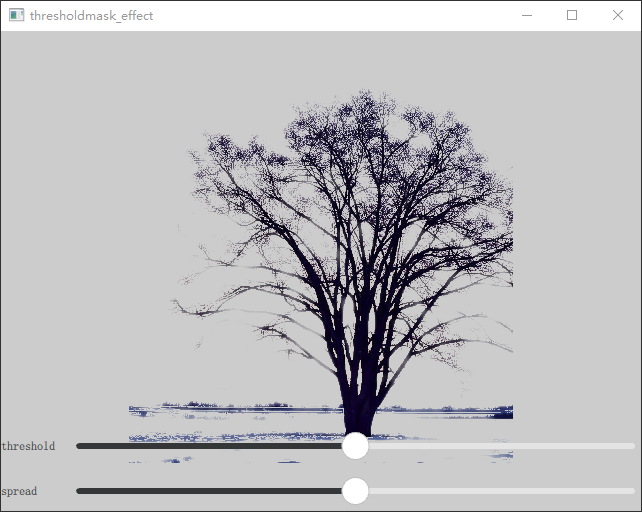
\includegraphics[width=0.95\textwidth]{../chapter06/thresholdmask_effect/the_app.png} %图片路径
\caption{ThresholdMask} %标题
\label{p000042} %索引
\end{figure}
%end图片


未完待续






%使用XeLaTeX编译
%版权所有,翻版必究
%本文件由程序自动生成,任何修改将被覆盖
%2019 年 01 月 23 日








% ______all_key_words
% the_book_chapter the_book_subsection the_book_subsubsection
% the_book_section the_book_image the_book_table
% the_book_file the_book_tree_file the_book_command_file
% littlelongworld tabbing ref
% figurename tablename filesourcenumbernameone
% treeindexnumbernameone commandnumbernameone footnote 
% item itemize comment textbullet
% \hspace*{\parindent}







%使用XeLaTeX编译
%版权所有,翻版必究
%本文件由程序自动生成,任何修改将被覆盖
%2019 年 01 月 23 日



